%%%%%%%%%%%%%%%%%%%%%%%%%%%%%%%%%%%%%%%%%
% MSc BIS Thesis 
% LaTeX Template
% Version 1.0 (29/08/2014)
%
% Original authors:
% Steven Gunn 
% Sunil Patel
%
% Further authors:
% Michael Stauffer
% 
% This template is based on
% http://www.latextemplates.com/template/masters-doctoral-thesis
%
% License:
% CC BY-NC-SA 3.0 (http://creativecommons.org/licenses/by-nc-sa/3.0/)
%
%%%%%%%%%%%%%%%%%%%%%%%%%%%%%%%%%%%%%%%%%

%----------------------------------------------------------------------------------------
%	PACKAGES AND OTHER DOCUMENT CONFIGURATIONS
%----------------------------------------------------------------------------------------

% For digital publication it is recommended to use a one-sided layout
\documentclass[11pt, oneside]{Thesis}
\addbibresource{Bibliography.bib}

% For printing it is recommended to use a two-sided layout
%\documentclass[11pt, twoside]{Thesis}

\makeglossaries

\begin{document}

%----------------------------------------------------------------------------------------
%	DOCUMENT VARIABLES
%	Fill in the lines below to update the thesis template
%	
%   If you want to cite each of the variables defined below, look at the
%	section above for the citation command.
%----------------------------------------------------------------------------------------

% You thesis title
% Citation command \thesisTitle
\thesisTitle{A Knowledge Graph and Large Language Model-Based Approach for Research Collaboration}
%-------------------------------------------------  

% You supervisor's name Unicam or FHNW
% Citation command \supName 
\supervisor{Dr. Emanuele \textsc{Laurenzi}}
%-------------------------------------------------  

% You supervisor's URL 
% Citation command \supURL
\supervisorURL{https://www.fhnw.ch/en/people/emanuele-laurenzi}
%-------------------------------------------------

% You supervisor's name Unicam or FHNW
% Citation command \supName 
\supervisorTwo{Prof. Michela \textsc{Quadrini}}

%-------------------------------------------------  

% You supervisor's URL
% Citation command \supURL
\supervisorTwoURL{https://computerscience.unicam.it/michela-quadrini}
%-------------------------------------------------


% If you don't have a co-supervisor, exchange with
\cosupervisorfalse
%\cosupervisortrue
%-------------------------------------------------

% You co-supervisor's name 
% Citation command \supcoName 
%\cosupervisor{Dr. James \textsc{Allan}}
%-------------------------------------------------  

% You co-supervisor's URL
% Citation command \supcoURL
\cosupervisorURL{https://www.empa.ch/web/alja}
%-------------------------------------------------

% Your degree name
% Citation command \degreeName
\degree{Business Information Systems}
\degreeTwo{Computer Science}
%-------------------------------------------------   

% Your name
% Citation command \authorName
\authors{Piermichele \textsc{Rosati}}
\matricola{124176}%
\academicyear{2023/2024}%
%-------------------------------------------------

% Your URL
% Citation command \authorURL
\authorsURL{http://www.johnsmith.com}
%-------------------------------------------------

% Your address (not used)
% Citation command \addressNames
\addresses{}
%-------------------------------------------------

% Your subject area (not used) 
% Citation command \subjectName
\subject{}
%-------------------------------------------------   

% Keywords for your thesis (not used)
% Citation command \keywordNames 
\keywords{}
%-------------------------------------------------

% http://www.fhnw.ch
% Citation command \fhnwURL 
%-------------------------------------------------

% University of Applied Sciences and Arts Northwestern Switzerland
% Citation command \fhnw 
%-------------------------------------------------

% UNIVERSITY OF APPLIED SCIENCES AND ARTS NORTHWESTERN SWITZERLAND
% Citation command \FHNW 
%-------------------------------------------------

% http://www.fhnw.ch/business
% Citation command \hswURL 
%-------------------------------------------------

% School of Business
% Citation command \hsw 
%-------------------------------------------------

% SCHOOL OF BUSINESS
% Citation command \HSW 
%-------------------------------------------------

% http://www.fhnw.ch/business/iwi
% Citation command \iwiURL 
%-------------------------------------------------

% Institute for Information Systems
% Citation command \iwi 
%-------------------------------------------------

% INSTITUTE FOR INFORMATION SYSTEMS for Information Systems
% Citation command \IWI
%-------------------------------------------------

%----------------------------------------------------------------------------------------
%	GLOSSARY
%	Add your glossary terms below
%	
%   If you want to cite a glossary term simply use \gls{term) for the singular form 
%   of the term or \glspl{term} for the plural form of the term.
%----------------------------------------------------------------------------------------

\newglossaryentry{Java}{
    name={Java},
    description={\blindtext}
}

\newglossaryentry{Oracle}{
    name={Oracle},
    description={\blindtext}
}

\newglossaryentry{Microsoft}{
    name={Microsoft},
    description={\blindtext}
}

%----------------------------------------------------------------------------------------
%	ABBREVIATIONS
%	Add your glossary terms below
%	
%   To generate the list of abbreviations run the following command in the terminal:
%   makeglossaries Rosati-2024-Thesis 
%
%   If you want to cite an abbreviation term simply use \gls{term) for the singular form  
%   of the term or \glspl{term} for the plural form of the term.
%----------------------------------------------------------------------------------------

\newacronym{rq}{RQ}{Research Question}
\newacronym{kg}{KG}{Knowledge Graph}
\newacronym{ai}{AI}{Artifical Intelligence}
\newacronym{llm}{LLM}{Large Language Model}
\newacronym{dnn}{DNN}{Deep Neural Network}
\newacronym{gnn}{GNN}{Graph Neural Network}
\newacronym{ml}{ML}{Machine Learning}
\newacronym{dl}{DL}{Deep Learning}
\newacronym{cnn}{CNN}{Convolutional Neural Network}
\newacronym{rnn}{RNN}{Recurrent Neural Network}
\newacronym{rdf}{RDF}{Resource Description Framework}
\newacronym{rdfs}{RDFS}{RDF Schema}
\newacronym{uri}{URI}{Uniform Resource Identifier}
\newacronym{owl}{OWL}{Web Ontology Language}
\newacronym{sparql}{SPARQL}{SPARQL Protocol and RDF Query Language}
\newacronym{nlp}{NLP}{Natural Language Processing}
\newacronym{lod}{LOD}{Linked Open Data}
\newacronym{kge}{KGE}{Knowledge Graph Embedding}
\newacronym{gcn}{GCN}{Graph Convolutional Network}
\newacronym{gat}{GAT}{Graph Attention Network}
\newacronym{mpnn}{MPNN}{Message Passing Neural Network}
\newacronym{graphsage}{GraphSAGE}{Graph Sample and Aggregation}
\newacronym{stgnn}{STGNN}{Spatio-Temporal Graph Neural Network}
\newacronym{tgn}{TGN}{Temporal Graph Networks}
\newacronym{lstm}{LSTM}{Long Short-Term Memory}
\newacronym{gru}{GRU}{Gated Recurrent Unit}
\newacronym{grnn}{GRNN}{Graph Recurrent Neural Network}
\newacronym{gae}{GAE}{Graph Autoencoder}
\newacronym{rgcn}{R-GCN}{Relational Graph Convolutional Network}
\newacronym{hran}{HRAN}{Heterogeneous Relation Attention Network}
\newacronym{mugnn}{MuGNN}{Multi-channel Graph Neural Network}
\newacronym{trar}{TRAR}{Target Relational Attention-Oriented Reasoning}
\newacronym{dpmpn}{DPMPN}{Dynamic Pruned Message Passing Networks}
\newacronym{hgcn}{H-GCN}{Hierarchical Graph Convolutional Network}
\newacronym{hdgi}{HDGI}{Heterogeneous Deep Graph Infomax}
\newacronym{han}{HAN}{Heterogeneous Graph Attention Networks}
\newacronym{cv}{CV}{Computer Vision}
\newacronym{w3c}{W3C}{World Wide Web Consortium}
\newacronym{mag}{MAG}{Microsoft Academic Graph}
\newacronym{s2ag}{S2AG}{Semantic Scholar Academic Graph}
\newacronym{orkg}{ORKG}{Open Research Knowledge Graph}
\newacronym{foaf}{FOAF}{Friend of a Friend}
\newacronym{doi}{DOI}{Digital Object Identifier}
\newacronym{orcid}{ORCID}{Open Researcher and Contributor ID}
\newacronym{viaf}{VIAF}{Virtual International Authority File}
\newacronym{cbf}{CBF}{Content-Based Filtering}
\newacronym{cf}{CF}{Collaborative Filtering}
\newacronym{gbc}{GBC}{Gradient Boosted Classifier}
\newacronym{auc}{AUC}{Area Under the Curve}
\newacronym{rag}{RAG}{Retrieval-Augmented Recommendation}

% PDF meta-data
\hypersetup{pdftitle={\thesisTitle}}
\hypersetup{pdfsubject=\subjectName}
\hypersetup{pdfauthor=\authorName}
\hypersetup{pdfkeywords=\keywordNames}

\frontmatter % Use roman page numbering style (i, ii, iii, iv...) for the pre-content pages

%----------------------------------------------------------------------------------------
%	TITLE PAGE
%----------------------------------------------------------------------------------------

\titlePage

%----------------------------------------------------------------------------------------
%	ABSTRACT PAGE
%----------------------------------------------------------------------------------------

\abstract{
    The Thesis Abstract is written here (and usually kept to just this page)\ldots
}

\clearpage % Start a new page

%----------------------------------------------------------------------------------------
%	STATEMENT OF AUTHENTICITY
%----------------------------------------------------------------------------------------

\fillingPage{} 
%\statementOfAuthenticity

\clearpage

%----------------------------------------------------------------------------------------
%	TABLE OF CONTENTS
%----------------------------------------------------------------------------------------

\tableofcontents

%----------------------------------------------------------------------------------------
%	THESIS CONTENT - CHAPTERS
%----------------------------------------------------------------------------------------

\mainmatter % Begin numeric (1,2,3...) page numbering

\fillingPage{}
\chapter{Introduction}\label{chap:intro}

This chapter presents the foundation of the thesis including the background, challenges, and goals of the study.
It begins with the Background (Sec. \ref{sec:background}), which provides an overview of research collaboration, its importance in advancing scientific discovery, and the role of digital tools and recommender systems in facilitating such collaborations.
The chapter then moves to the Problem Statement (Sec. \ref{sec:problem-statement}), highlighting the limitations of traditional approaches and existing \gls{ai} methods in identifying potential research collaborators, such as their lack of interpretability, contextual understanding, and ability to generalize across diverse scenarios.
Sec. \ref{sec:thesis-statement} defines the Thesis Statement, which outlines the proposed solution: a recommender system integrating knowledge graphs and large language models to deliver accurate, explainable, and context-aware recommendations.
The Research Gap (Sec. \ref{sec:research-gap}) identifies shortcomings in current methods, emphasizing the unexplored potential of combining knowledge graphs with retrieval-augmented large language models to enhance precision and explainability.
The chapter also illustrates Research Questions (Sec. \ref{sec:research-questions}) to guide the investigation and concludes with a Thesis Structure (Sec. \ref{sec:thesis-structure}), offering a roadmap for the subsequent chapters of the document.

\section{Background}\label{sec:background}
Research collaboration is the process where researchers from various fields, institutions, or disciplines work together to achieve shared scientific objectives (\cite{KATZ19971}).
The exponential growth of academic research in various fields has increased the need for effective collaboration between researchers (\cite{Adams2012, Vermeulen2017}).
Research collaborations are commonly used in areas such as medicine, engineering, social sciences, and environmental studies, where diverse expertise is often required to tackle intricate problems.
According to \cite{Mei2021}, these collaborations are vital for addressing complex, multidisciplinary challenges, advancing knowledge, and accelerating innovation.
They typically take the form of joint publications, shared research grants, co-developed methodologies, and interdisciplinary studies.
Their importance is underscored by their ability to share resources and knowledge and foster innovation, making them key factors in scientific progress.

Traditional approaches to collaboration often rely on professional networking through conferences, workshops, and institutional partnerships (\cite{KATZ19971}).
These methods have proven effective in facilitating connections, but are often constrained by geographic and logistical limitations.
Digital tools, such as ResearchGate\footnote{\url{https://www.researchgate.net}}, Academia.edu\footnote{\url{https://www.academia.edu}}, Google Scholar\footnote{\url{https://scholar.google.com}} and LinkedIn\footnote{\url{https://www.linkedin.com}}, have expanded the reach of collaborations, allowing researchers to network online, share results, and identify potential collaborators around the world.
However, these platforms focus primarily on social connectivity rather than intelligent matchmaking based on complementary expertise or shared goals.

Recommender systems (\cite{Lu2012}) are \gls{ai} algorithms that make suggestions and recommendations about the most relevant items for a particular user.
Nowadays, they are widely used in commercial contexts such as e-commerce and streaming platforms and have shown significant potential to address the challenge of matching individuals with relevant objects or entities (\cite{Hussien2021}).

In recent years, area of \gls{ai} such as \gls{ml} and \gls{dl} algorithms,  \glspl{kg}, and \glspl{llm} have emerged as powerful tools for developing intelligent and interpretable recommendation systems (\cite{Zhao2024}).
\glspl{kg} enable the representation of structured information about entities and their relationships, providing a basis for reasoning and generating insights.
At the same time, \glspl{llm} have demonstrated remarkable abilities to process and understand complex textual information. 

The Semantic Web, an extension of the World Wide Web for enhancing the current web plays a crucial role in this context.
By embedding structured, machine-readable data into web resources, the Semantic Web allows information to be interconnected and queried seamlessly across diverse datasets.
Standards such as the \gls{rdf} (\cite{Cyganiak14RCA}) and \gls{owl} (\cite{Deborah2004}) form the foundation of the Semantic Web, enabling interoperability and integration of data from various sources.
These capabilities are particularly valuable for applications requiring complex reasoning and decision-making.

The combination of advanced \gls{ai} methodologies with Semantic Web technologies has opened new possibilities for enhancing recommender systems.
By leveraging the structured, interconnected data of the Semantic Web alongside the predictive power of \gls{ai} algorithms, these systems can deliver more accurate, relevant, and context-aware recommendations.
This not only improves the effectiveness of recommender systems but also expands their potential to address the sophisticated requirements of users in academic and scientific collaboration settings.
%
\section{Problem Statement}\label{sec:problem-statement}

Research collaboration is an essential part of modern scientific progress, but it presents many challenges that make it difficult to be effective.
A significant problem comes from disciplinary and cognitive differences: collaborators from different fields often struggle to reconcile conflicting methodologies, priorities, and theoretical perspectives.
Communication barriers further make these challenges more difficult, as insufficient or ineffective exchanges between team members can lead to misunderstandings and a lack of cohesion.
Inconsistent levels of commitment within teams often create imbalances, with some researchers prioritizing their personal goals over collective ones, thus straining trust and productivity.
In addition, disputes over equity, such as work distribution, authorship, and access to resources, can lead to employee dissatisfaction and resentment.
Ineffective leadership and management practices, such as overregulation or lack of flexibility, often fail to adequately address these problems or may even intensify them.
Cultural and social differences, including variations in organizational norms, gender, or cultural background, while potentially enriching collaboration, can also generate friction if not managed inclusively.


\glspl{dnn} have achieved remarkable progress in enhancing recommender systems by modeling user-item interactions and incorporating textual side information.
These systems are very good at capturing patterns and preferences from large datasets, often leading to state-of-the-art performance in recommendation tasks.
However, despite these advancements, \gls{dnn}-based recommender systems have several limitations:
\begin{enumerate}
    \item Understanding users' interests: \glspl{dnn} often struggle to effectively comprehend users' intricate and evolving interests, particularly in highly dynamic domains such as academic research.
    \item Capturing textual side information: while incorporating textual data such as abstracts, keywords, or titles, \glspl{dnn} may fail to adequately integrate this information into the recommendation process due to limitations in contextual understanding.
	\item Generalization challenges: \gls{dnn}-based systems face difficulties in generalizing across various seen and unseen recommendation scenarios, reducing their applicability in real-world settings with sparse or incomplete data.
	\item Lack of interpretability: \glspl{dnn} are often criticized for their black-box nature, making it challenging to provide meaningful explanations for recommendations and undermining user trust in the system.
\end{enumerate}
		

These challenges underscore the need for more sophisticated methods that integrate domain-specific knowledge, facilitate reasoning, and provide interpretable recommendations in specific contexts, such as research collaboration.
%
\section{Thesis Statement}\label{sec:thesis-statement}

This thesis proposes the design and development of a recommendation system that leverages the power of \glspl{kg} and \glspl{llm} to provide accurate and explainable recommendations for identifying potential research collaborators.
By integrating \glspl{kg}, which provide a structured and interconnected representation of domain-specific information, with the contextual understanding and generative capabilities of \glspl{llm}, the system aims to address key challenges of research collaboration recommendations.
These include understanding complex academic relationships, the research consortia and projects and areas of interest of researchers, and explaining the motivations behind recommendations.
The proposed system leverage the strengths of both technologies to retrieve and analyze relevant academic data, dynamically adapt to user preferences, and provide personalized and well-justified recommendations, thus enhancing the process of finding and connecting with suitable research collaborators.
%
\section{Research Gap}\label{sec:research-gap}
Despite significant advancements in \gls{dl} models for recommender systems, these models exhibit critical limitations in capturing the nuanced preferences and diverse textual side information of users.
They often struggle with generalizing to unseen recommendation scenarios and explaining the reasoning behind their predictions \cite{Zhao2024}.
This lack of explainability and adaptability reduces their effectiveness in tasks requiring complex reasoning, such as research collaborator recommendations.

\glspl{llm} have emerged as transformative tools due to their exceptional natural language understanding and generation capabilities, enabling them to grasp complex patterns and provide human-like reasoning.
When combined with \gls{rag}, \glspl{llm} can overcome the limitations of \gls{dl} models by integrating external knowledge sources, reducing hallucinations, and providing contextually enriched, explainable, and accurate recommendations \cite{Deldjoo2024}.

This combination represents a promising avenue for addressing the challenges of explainability and precision in recommending research collaborators, particularly by aligning recommendations with explicit user queries and leveraging diverse, up-to-date knowledge bases.
However, the integration of \glspl{llm} and \gls{rag} in this specific context remains underexplored, presenting an opportunity to bridge this gap and advance the field.
%
\section{Research Questions}\label{sec:research-questions}
The main \gls{rq} is derived from the thesis statement and guides the investigation:

\textit{How can a \gls{kg} and \gls{llm}-based approach enhance the process of suggesting research collaborators for researchers?}

To address this question, the following subquestions are explored:
\begin{itemize}
	\item Awareness of the problem: \textit{how can research-related data (e.g., publications, topics, affiliations) be effectively modeled into a \gls{kg} to capture relationships among researchers?}
	\item Suggestions: \textit{How can a \gls{kg} and \gls{llm}-based system be designed to efficiently retrieve relevant information from large, heterogeneous data sources to support personalized recommendations?}
	\item Implementation: \textit{How can the system generate human-readable explanations for its research collaborator recommendations using the \gls{kg} and \gls{llm} outputs?}
\end{itemize}

%\begin{itemize}
%    \item Knowledge Representation: \textit{how can research-related data (e.g., publications, topics, affiliations) be effectively modeled into a \gls{kg} to capture relationships among researchers?}
%	\item Information Retrieval: \textit{What techniques can be employed to efficiently retrieve relevant information from large, heterogeneous data sources to support personalized recommendations?}
%	\item Explainability: \textit{How can the system generate human-readable explanations for its recommendations using the \gls{kg} and \gls{llm} outputs?}
%	\item Evaluation: \textit{What metrics and evaluation frameworks are suitable to assess the accuracy, usability, and satisfaction of the proposed system?}
%\end{itemize}

By addressing these questions, this thesis aims to contribute to the field of intelligent recommender systems and facilitate impactful research collaborations.

\section{Thesis Structure}\label{sec:thesis-structure}
TODO
%Chapter \ref{chap:literature-review} provides an overview of the relevant literature on \glspl{kg}, \glspl{gnn}, and \glspl{llm}, as well as related work on research collaboration recommendation systems;
%Chapter \ref{chap:research-method} outlines the methodology used to design and implement the proposed system;
%Finally \ref{chap:conclusion} concludes the thesis and discusses potential future research directions.

 
\fillingPage{}
\chapter{Literature Review}\label{chap:literature-review}

As part of the problem awareness phase, the literature review summarises the relevant scientific literature related to the topics of this thesis.
It lays the groundwork for answering to the research questions.
Initially, Sec.~\ref{sec:research-collaboration} discusses the definition and importance of research collaboration and methods for finding potential research collaborators.
Sec.~\ref{sec:knowledge-graphs} provides an overview of knowledge graphs, from theoretical aspects to real-world applications.
Existing knowledge graphs and ontologies in the research field are also described.
Sec.~\ref{sec:large-language-models} briefly provides an overview of \glspl{llm}, applications of these technologies with their advantages and limitations.
Finally, Sec.~\ref{sec:recommender-systems} explains recommendation systems, particularly existing recommendation systems in the search domain and \gls{rag}-based recommendation systems.
%
\section{Research Collaboration}\label{sec:research-collaboration}
\subsection*{Definition and Importance of Research Collaboration}
\cite{Bozeman2014} define research collaboration as the process in which individuals pool their skills, knowledge, and resources to generate new scientific insights and address complex challenges.
It has been described as a social process that combines human capital, such as formal training and technical skills, with social capital, including networks and collaborative relationships, to advance knowledge creation (\cite{Bozeman2014}).
This collaboration often takes place within the framework of ``team science'', where interdisciplinary teams work collectively to tackle multifaceted problems that surpass the scope of single-discipline research.
Within research collaboration, the goals can range from knowledge-based objectives, such as publishing academic articles and creating educational resources, to property-based outcomes, including patents and commercial technologies.

Co-authorship is frequently used as a tangible indicator of collaboration, though it only captures a fraction of the collaborative efforts that occur in scientific work.

Boundary-spanning collaborations, such as those crossing institutional, disciplinary, or sectoral lines, are particularly crucial for addressing global challenges but require careful alignment of goals and effective communication to overcome cultural and operational differences.

Despite its significant benefits, research collaboration is often impeded by challenges such as disciplinary silos, communication barriers, and logistical constraints.
As collaboration becomes increasingly essential in the era of team science and global research, understanding these dynamics is critical for fostering effective partnerships and advancing scientific discovery.

\cite{KATZ19971} define the term research collaboration refers to the process where researchers from various disciplines, institutions, or regions work together toward shared objectives.
It plays a critical role in advancing scientific knowledge, addressing complex challenges, and fostering innovation.
Collaborative efforts enable the pooling of diverse expertise, resources, and perspectives, which are essential for tackling interdisciplinary problems (\cite{KATZ19971}).
The increasing prevalence of co-authored publications and large-scale projects underscores the importance of collaboration in modern academia (\cite{Adams2012}).

\subsection*{Methods to Find Research Collaborators}
Identifying suitable collaborators is a foundational step in establishing successful research partnerships.
Finding a potential research collaborator often relies on various methods, with personal and professional networking being among the most prominent.
According to \cite{KATZ19971}, traditional approaches like conferences, workshops, and seminars provide researchers with opportunities to establish connections and build trust, which is critical for reducing the transaction costs of collaboration and enhancing its overall effectiveness.
These face-to-face interactions create a foundation for partnerships by fostering mutual understanding and shared interests, especially in multidisciplinary fields (\cite{Bozeman2014}).

Institutional and organizational connections also play a significant role in facilitating collaborations. Universities and research centers often promote partnerships through formal agreements or structured programs, giving researchers access to a broader network of professionals and shared resources. These institutional linkages help bridge gaps between disciplines or organizations, enabling researchers to leverage collective expertise and infrastructure.

Trust and social capital are fundamental factors in initiating and sustaining collaborations. Collaborations often emerge from prior acquaintance or existing professional relationships, where trust reduces the perceived risks and uncertainties involved in working together. This trust is particularly vital in interdisciplinary or inter-institutional collaborations, where differences in methodologies, goals, or organizational cultures might otherwise hinder progress (\cite{Bozeman2014}).

Additionally, recommendations from colleagues, mentors, or supervisors often serve as effective means of identifying potential collaborators.
These recommendations draw on the existing trust and knowledge of the recommender, providing a reliable basis for collaboration (\cite{Bozeman2014}).

Ultimately, the success of research collaboration depends on key factors such as the alignment of research goals, complementary expertise, effective communication, and the ability to navigate cultural or disciplinary differences.
By leveraging these methods and addressing these factors, researchers can establish productive and enduring partnerships (\cite{Bozeman2014}).

Digital platforms have increasingly become essential tools for finding collaborators. Online academic networks, citation databases, and digital communities allow researchers to search for potential collaborators based on shared research interests, publication records, or complementary expertise. These platforms have expanded the reach of collaborations, making it easier for researchers to connect globally and explore new opportunities.
However, these methods often require researchers to actively seek and evaluate potential collaborators, which can be time-intensive and subjective.
%
\section{Knowledge Graphs}\label{sec:knowledge-graphs}
\glspl{kg} have came up as a key technology in the field of data management and \gls{ai}, enabling sophisticated data integration, retrieval and analysis, and analysis.
This section provides an in-depth examination of \glspl{kg}, their theoretical foundations, practical applications and recent advances.

\subsection*{Theoretical Foundations of Knowledge Graphs}
\subsubsection*{Definition and Structure}
\glspl{kg} are directed graph-based data structures that represent real-world entities and their interrelations, providing a way to model complex domains and their underlying semantics.
A \gls{kg} consists of nodes (also called entities) and edges (also called relationships), forming a network of interconnected information.
This structure allows \glspl{kg} to capture rich contextual information and provide a semantic framework for data (\cite{Hogan2021}).
In other words, a \gls{kg} refers to a semantic network graph which is consisted of diverse entities, concepts, and relationships.
It is used to formally describe various things and their associations in the real world.
\glspl{kg} are generally represented in triples $\gls{kg}=\{\mathnormal{E,R,F}\}$.
\begin{itemize}
    \item $E$ represents the entity set $\{\mathnormal{e_1, e_2, ... ,e_E} \}$, and the entity $e$ is the most basic element in the \gls{kg}, referring to the items that exist objectively and can be distinguished from each other.
    \item $R$ represents the relation set $\{\mathnormal{r_1, r_2, ... ,r_R}\}$, and the relation $r$ is an edge in the \gls{kg}, representing a specific connection between different entities.
    \item $F$ represents the fact set $\{\mathnormal{f_1,f_2, ... ,f_F}\}$, and each $\mathnormal{f}$ is defined as a triple $(\mathnormal{h,r,t}) \in \mathnormal{f}$, in which $\mathnormal{h}$ denotes the head entity, $\mathnormal{r}$ stands for the relationship, and $\mathnormal{t}$ indicates the tail entity.
\end{itemize}

The \gls{kg} in Fig. \ref{fig:kg-example-albert-einstein} visually represents some relationships and attributes associated with Albert Einstein.
At the center of the graph is ``Albert Einstein'', from which several connections extend.
One connection indicates that he was ``born in'' Germany.
Another connection shows his ``occupation'' as a ``Theoretical Physicist''.
This occupation is further connected to ``Physicist'' as a ``kind of'' category, indicating that a theoretical physicist is a type of physicist.
The graph also shows that a physicist ``practices'' physics.
Additionally, it highlights that Albert Einstein ``developed'' the ``Theory of Relativity'', which is shown as a ``branch of'' physics.
The graph effectively maps out key aspects of Albert Einstein's background, profession, and contributions to science.

\begin{figure}[htbp]
    \centering
 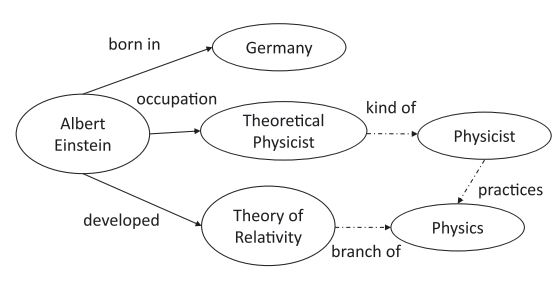
\includegraphics[width=.7\textwidth]{03_Figures/literature-review/kg-example-albert-einstein.png}
     \rule{35em}{0.5pt}
    \caption{An example of \acrlong{kg} (\cite{Chaudhri2022})} 
 \label{fig:kg-example-albert-einstein}
\end{figure}

\subsubsection*{Ontologies and Semantic Web Technologies}
An ontology is a formal representation of knowledge in a domain, specifying the concepts, relationships, and constraints that exist within that domain. The term ``ontology'' can be used to the shared understanding of some domain of interest (\cite{Uschold1996}).
Ontologies play a critical role in defining the schema and semantics of \glspl{kg}. They specify the types of entities, relationships, and constraints, thereby providing a formalized structure for the data. The Semantic Web technologies, particularly the \gls{rdf} and the \gls{owl}, are fundamental to the development and functioning of \glspl{kg} (\cite{Antoniou2008}).
\\\gls{rdf} is a standard model for data interchange on the web.
\gls{rdf} is a part of the \gls{w3c}'s Semantic Web activity and provides a model for data interchange on the Web.
It uses triples $\langle subject,predicate,object \rangle$ to represent information, providing a flexible and extensible framework for creating and managing \glspl{kg} (\cite{Cyganiak14RCA}).
The subject is the resource being described, the predicate is the property or characteristic of the subject, and the object is the value of the property, that can be literals, which are concrete data values such as strings, numbers, or dates..
\gls{rdf} uses \glspl{uri} to uniquely identify subjects and predicates, ensuring that resources are globally identifiable.
\gls{rdf} can be serialized in various syntaxes, including \gls{rdf}/XML, Turtle, N-Triples, and JSON-LD. \gls{rdf}/XML is the original \gls{rdf} syntax using XML to represent \gls{rdf} triples. Turtle is a more human-readable syntax for \gls{rdf} data, concise and easier to write and read compared to \gls{rdf}/XML. N-Triples is a plain text format for encoding \gls{rdf} triples, useful for streaming data or simple data exchange. JSON-LD is a JSON-based format to serialize Linked Data, designed to be easy to use and integrate with existing JSON-based systems.
\gls{rdfs} is a semantic extension of \gls{rdf} that provides mechanisms to describe groups of related resources and the relationships between these resources. It allows for defining classes, which are categories of resources; properties, which are relationships between resources; and hierarchies, enabling inheritance.
\gls{rdf} is widely used in various domains, including the Semantic Web, where it enables the creation of a web of data with meaning, allowing machines to understand and process web content; \glspl{kg}, powering large-scale graph-based data structures used by organizations like Google and Amazon (\cite{Kejriwal2022}); data integration, integrating data from disparate sources by providing a common data model; and ontology engineering, defining and using ontologies to model domain knowledge. \gls{rdf} provides a robust and flexible framework for representing structured information, enabling interoperability and integration of data across different systems and domains.
\\\gls{owl} is used to explicitly represent the meaning of terms in vocabularies and the relationships between those terms. It enables more complex and expressive representations compared to \gls{rdfs} (\cite{Deborah2004}).
The \gls{owl} standard is a \gls{w3c} technology for defining and using web ontologies, enhancing \gls{rdf} by offering greater expressiveness for complex information. \gls{owl} ontologies consist of classes, properties, and individuals, enabling detailed descriptions of relationships and characteristics. It supports complex class expressions, including logical operators and restrictions like cardinality and property constraints.
\gls{owl} has three sublanguages: \gls{owl} Lite (simple feature set), \gls{owl} DL (maximum expressiveness with computational guarantees), and \gls{owl} Full (greatest expressiveness without computational guarantees). Reasoning capabilities in \gls{owl} allow for inferring implicit knowledge, consistency checking, and classification.
\gls{owl} is used in knowledge management, information integration, and semantic search, providing a common framework for understanding and integrating data. It promotes interoperability and the creation of semantically rich, interconnected web data.

\subsubsection*{Query Languages}
\gls{sparql} is the standard query language for retrieving and manipulating data stored in \gls{rdf} format. It allows users to write complex queries to extract specific information from a \gls{kg}, making it a powerful tool for data analysis and knowledge discovery (\cite{Jorge2009}).
It allows users to query \gls{rdf} data by specifying patterns of triples and to update \gls{rdf} data by inserting, deleting, and modifying \gls{rdf} triples. \gls{rdf} is a foundation for Linked Data, which involves interlinking data across the web using \glspl{uri} and \gls{rdf}. This enables the creation of a web of data that can be easily connected and queried.

Cypher is another query language for graph databases, such as Neo4j, that allows users to interact with graph data using a pattern-matching syntax. Cypher queries are used to traverse the graph, retrieve specific patterns, and perform operations on the data (\cite{Francis2018}).
Cypher supports complex queries involving multiple nodes and relationships, aggregation, sorting, and limiting results. It also provides functions for working with strings, numbers, dates, and collections, as well as support for subqueries and variable-length paths.
Cypher is widely used for graph analytics, network analysis, and data exploration, enabling users to easily express complex graph traversals and operations. It leverages Neo4j's indexing and optimization capabilities to ensure efficient execution of queries, making it a powerful tool for working with connected data.

\subsection*{Applications of Knowledge Graphs}

\subsubsection*{General Applications}
\glspl{kg} have been adopted across various domains due to their ability to integrate heterogeneous data sources, provide semantic context, and enable advanced querying and reasoning.
According to \cite{Kapanipathi2020}, in healthcare \glspl{kg} are used to integrate patient records, clinical trials, research data, and medical ontologies, enabling personalized medicine and decision support systems. They help in identifying relationships between diseases, treatments, and patient outcomes.
\\Financial institutions leverage \glspl{kg} to connect data from various sources, such as market data, regulatory information, and customer transactions. This integration facilitates risk management, fraud detection, and compliance monitoring (\cite{Tchechmedjiev2019}).
\\In e-commerce, \glspl{kg} enhance product recommendation systems by linking customer preferences, purchase history, and product information. They enable more personalized and relevant recommendations, improving customer satisfaction and sales (\cite{Zhang2021}).

In compliance with \cite{Zou2020}, Fig. \ref{fig:kg-application-fields} shows a mind map illustrating the main applications of knowledge graphs. It divides the applications into five main categories: question answering, recommendation systems, information retrieval, domain-specific applications and other applications. With regard to question answering, methods based on semantic parsing, methods based on information retrieval, methods based on embedding, methods based on \gls{dl} and more complex tasks are included.
\glspl{kg} significantly enhance search engines by providing semantic search capabilities. They enable the understanding of user queries in context, allowing for more accurate and relevant search results. Google's Knowledge Graph is a prominent example, enhancing search results with information about entities and their relationships (\cite{singhal2012introducing}).
Recommender systems are classified into embedding-based methods, path-based methods and other methods. Information retrieval includes query representation, document representation, ranking and \gls{dl}. Domain-specific applications include medicine, computer security, finance, news and education.
Within enterprises, \glspl{kg} are used to manage and utilize internal knowledge effectively. They integrate data from different departments, such as human resources, finance, and operations, providing a unified view of the organization's information. This integration supports decision-making, collaboration, and innovation (\cite{pujara2013knowledge}).
Other applications include social networks, classification, geosciences and various other applications.

\begin{figure}[htbp]
	   \centering
    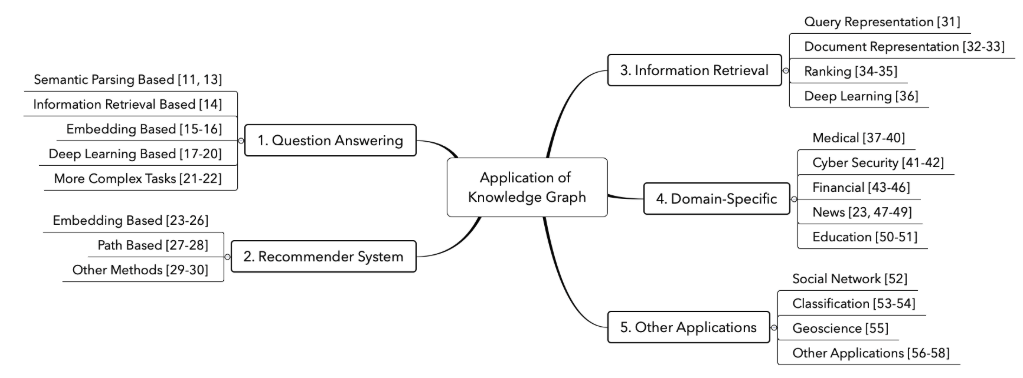
\includegraphics[width=\textwidth]{03_Figures/literature-review/kg-application-fields.png}
		\rule{35em}{0.5pt}
	   \caption{Application of \acrlongpl{kg} (\cite{Zou2020})} 
    \label{fig:kg-application-fields}
\end{figure}

\subsection*{Recent Advancements in Knowledge Graphs}

\subsubsection*{Integration with Machine Learning}
Recent research has focused on integrating \glspl{kg} with \gls{ml} and \gls{dl} techniques to enhance their capabilities and applications. These integrations have led to significant advancements in various areas, including \gls{nlp}, recommendation systems, and predictive analytics.
\begin{itemize}
    \item \textbf{\glspl{kge}}: \gls{kge} techniques represent entities and relationships in a continuous vector space, enabling the use of \gls{ml} algorithms for tasks such as link prediction, entity classification, and clustering. Popular methods include TransE (\cite{Bordes2013}), TransH (\cite{Wang2014}), and TransR (\cite{Lin2015}), each providing different ways to model relationships in the embedding space (\cite{Wang2017}).
    \item \textbf{\glspl{gnn}}: \glspl{gnn} are \gls{dl} models designed to operate on graph-structured data. They leverage the relational nature of graphs to perform tasks such as node classification, link prediction, and graph classification. \glspl{gnn} have been successfully applied to enhance the capabilities of \glspl{kg} in various domains (\cite{Wu2021}).
    
    Section \ref{sec:graph-neural-networks} provides a comprehensive and in-depth description of \glspl{gnn}.
\end{itemize}

\subsubsection*{Natural Language Processing and Question Answering}
\glspl{kg} have been instrumental in advancing \gls{nlp} applications, particularly in question answering systems. By providing structured and semantically rich information, \glspl{kg} enable systems to understand and generate human language more effectively.
\glspl{kg} support question answering systems by enabling them to retrieve and reason over structured data.
These systems can answer complex queries by traversing the graph and applying logical inferences based on the relationships between entities (\cite{Yasunaga2021}).
\glspl{kg} enhance text analysis and semantic search by providing contextual information about entities mentioned in the text.
This contextual understanding improves the accuracy of information retrieval and the relevance of search results (\cite{Fernandez2011}).

\subsection*{Challenges and Future Directions}

\subsubsection*{Scalability and Performance}
As \glspl{kg} grow in size and complexity, scalability and performance become critical challenges. Efficient storage, querying, and updating of large \glspl{kg} require advanced techniques and architectures. Research in distributed computing, graph databases, and parallel processing is ongoing to address these issues (\cite{Chaudhri2022}).
 
\subsubsection*{Data Quality and Integration}

Ensuring the accuracy and consistency of data in \glspl{kg} is essential for their reliability. Data quality issues, such as inconsistencies, duplications, and inaccuracies, can significantly impact the performance of applications relying on \glspl{kg}. Developing methods for automatic data cleaning, validation, and integration is an active area of research (\cite{Paulheim2017}).

\subsubsection*{Privacy and Security}

The integration of sensitive data into \glspl{kg} raises concerns about privacy and security. Protecting personal and confidential information while allowing for meaningful data analysis is a significant challenge. Research is focusing on developing techniques for secure data sharing, access control, and anonymization within \glspl{kg} (\cite{Bonatti2017}).

\subsubsection*{Interoperability and Standardization}

Interoperability and standardization are crucial for the widespread adoption of \glspl{kg}. Ensuring that different \glspl{kg} can work together seamlessly and that their data can be easily integrated requires the development of common standards and protocols. Efforts such as the \gls{lod} initiative and \gls{w3c} standards aim to address these challenges (\cite{Bizer2023}).

\subsection*{Conclusion}
\glspl{kg} represent a transformative technology for data integration, retrieval, and analysis, offering significant benefits across various domains. Their ability to provide semantic context and capture complex relationships makes them invaluable for applications in healthcare, finance, e-commerce, and enterprise knowledge management. Recent advancements in \gls{ml}, particularly in the integration with \glspl{gnn}, have further enhanced the capabilities of \glspl{kg}, opening new avenues for research and application. However, challenges related to scalability, data quality, privacy, and interoperability remain and must be addressed to fully realize the potential of \glspl{kg}. Continued research and development in these areas will be crucial for the future evolution and adoption of \glspl{kg}.
%
\section{Large Language Models}\label{sec:large-language-models}
\glspl{llm} have emerged as a transformative innovation in \gls{nlp}, leveraging deep learning techniques to understand, generate, and manipulate human language with unprecedented accuracy.
Fig. \ref{fig:llms-over-the-years} shows the increasing trend in the number of \glspl{llm} releases and the names of some significant \glspl{llm} proposed from 2019 to 2024.

\begin{figure}[htbp]
    \centering
 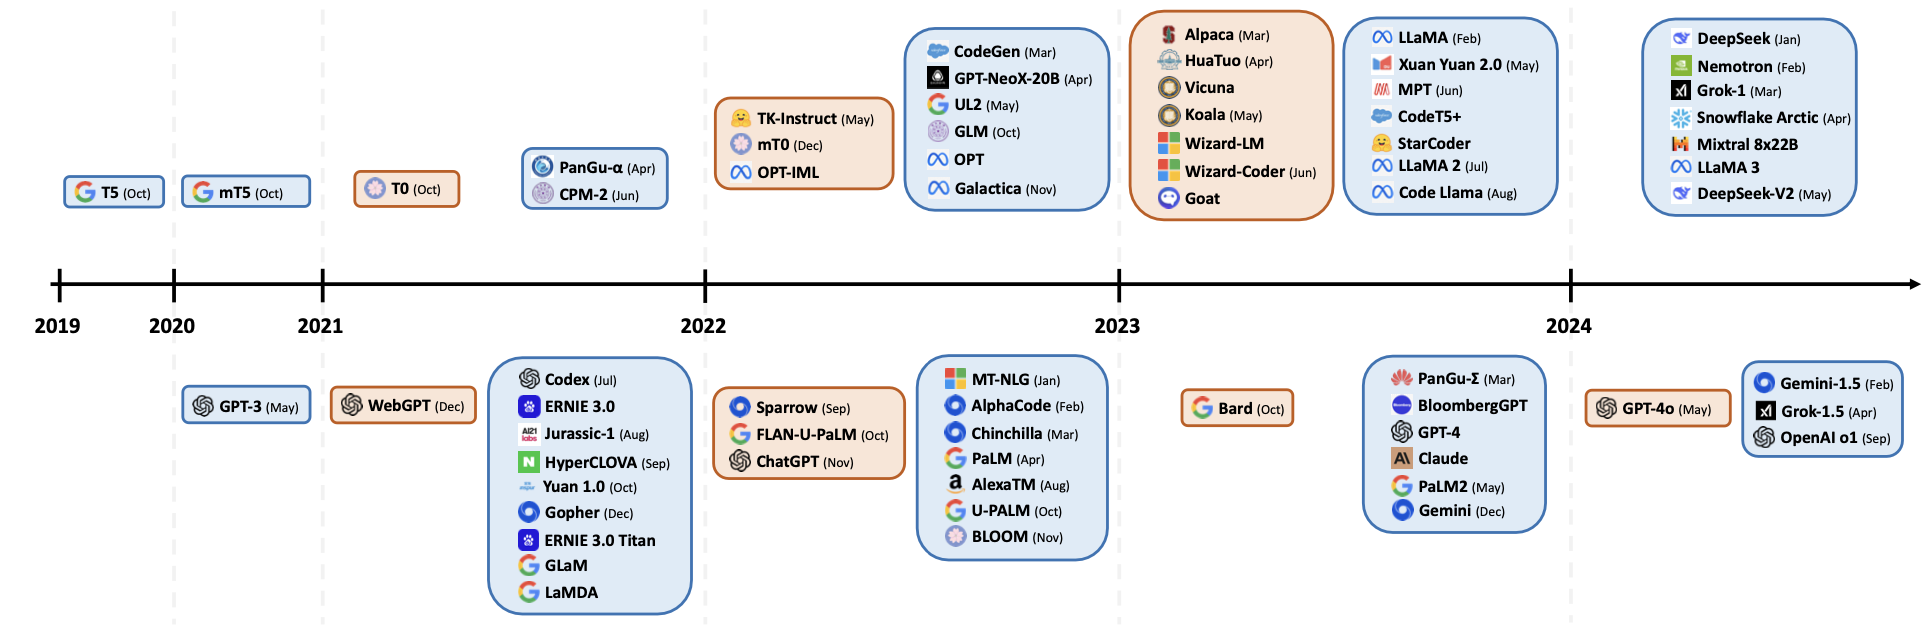
\includegraphics[width=\textwidth]{03_Figures/literature-review/llms-over-the-years.png}
     \rule{35em}{0.5pt}
    \caption{Timeline of \gls{llm} releases: blue cards represent pre-trained models, orange cards denote instruction-tuned models. Open-source models appear on the top, while closed-source models are on the bottom, showing the shift toward open-source and instruction-tuned trends. (\cite{Naveed2023})}
 \label{fig:llms-over-the-years}
\end{figure}

\glspl{llm}, such as OpenAI's GPT series (\cite{Radford2018ImprovingLU}), Google's BERT (\cite{Devlin2019BERTPO}), and more recent iterations like GPT-4, are typically built on transformer architectures (\cite{Vaswani2017}).
The transformer model introduced a self-attention mechanism that efficiently captures contextual relationships between words across large textual sequences, overcoming limitations of earlier models like \glspl{rnn} and \glspl{lstm} in handling long-range dependencies.
These models are pre-trained on massive corpora containing diverse text from books, articles, and web sources, allowing them to generalize linguistic patterns, syntax, semantics, and even factual knowledge embedded in the data.

According to \cite{Chang2024}, \glspl{llm} perform a wide range of tasks in \gls{nlp}, often achieving state-of-the-art results across various benchmarks.
Figure \ref{fig:llms-overview} provides a broader overview of the organization of \glspl{llm}, categorizing them into seven distinct branches: pre-training, fine-tuning, efficiency, inference, evaluation, applications, and challenges.
These branches reflect the key aspects of the development, deployment, and evaluation of \glspl{llm}.
Pre-training focuses on the foundational step of training models on vast, diverse corpora to learn language representations.
Fine-tuning involves adapting pre-trained models for specific tasks, enhancing their performance on downstream applications.
Efficiency addresses the computational and energy requirements of training and deploying \glspl{llm}, emphasizing methods like parameter-efficient tuning and pruning to reduce resource consumption.
The inference branch examines the process of generating outputs from trained models, focusing on optimizing speed and accuracy.
More advanced capabilities, such as few-shot and zero-shot learning, enable \glspl{llm} to adapt to new tasks with minimal to no task-specific training data, a feature prominently demonstrated by GPT-3 (\cite{NEURIPS2020_1457c0d6}).
Evaluation highlights the metrics and benchmarks used to assess \glspl{llm}' performance on various tasks, ensuring they meet quality standards.
Applications span the diverse real-world use cases of \glspl{llm}, from natural language understanding to robotics and multi-modal systems.
Finally, challenges encompass the limitations and issues of \glspl{llm}, including bias, hallucination, and environmental impact, offering directions for future research and improvement.
These branches collectively define the lifecycle and scope of advancements in \gls{llm} research, providing a comprehensive framework for understanding their capabilities and impact.

\begin{figure}[htbp]
    \centering
 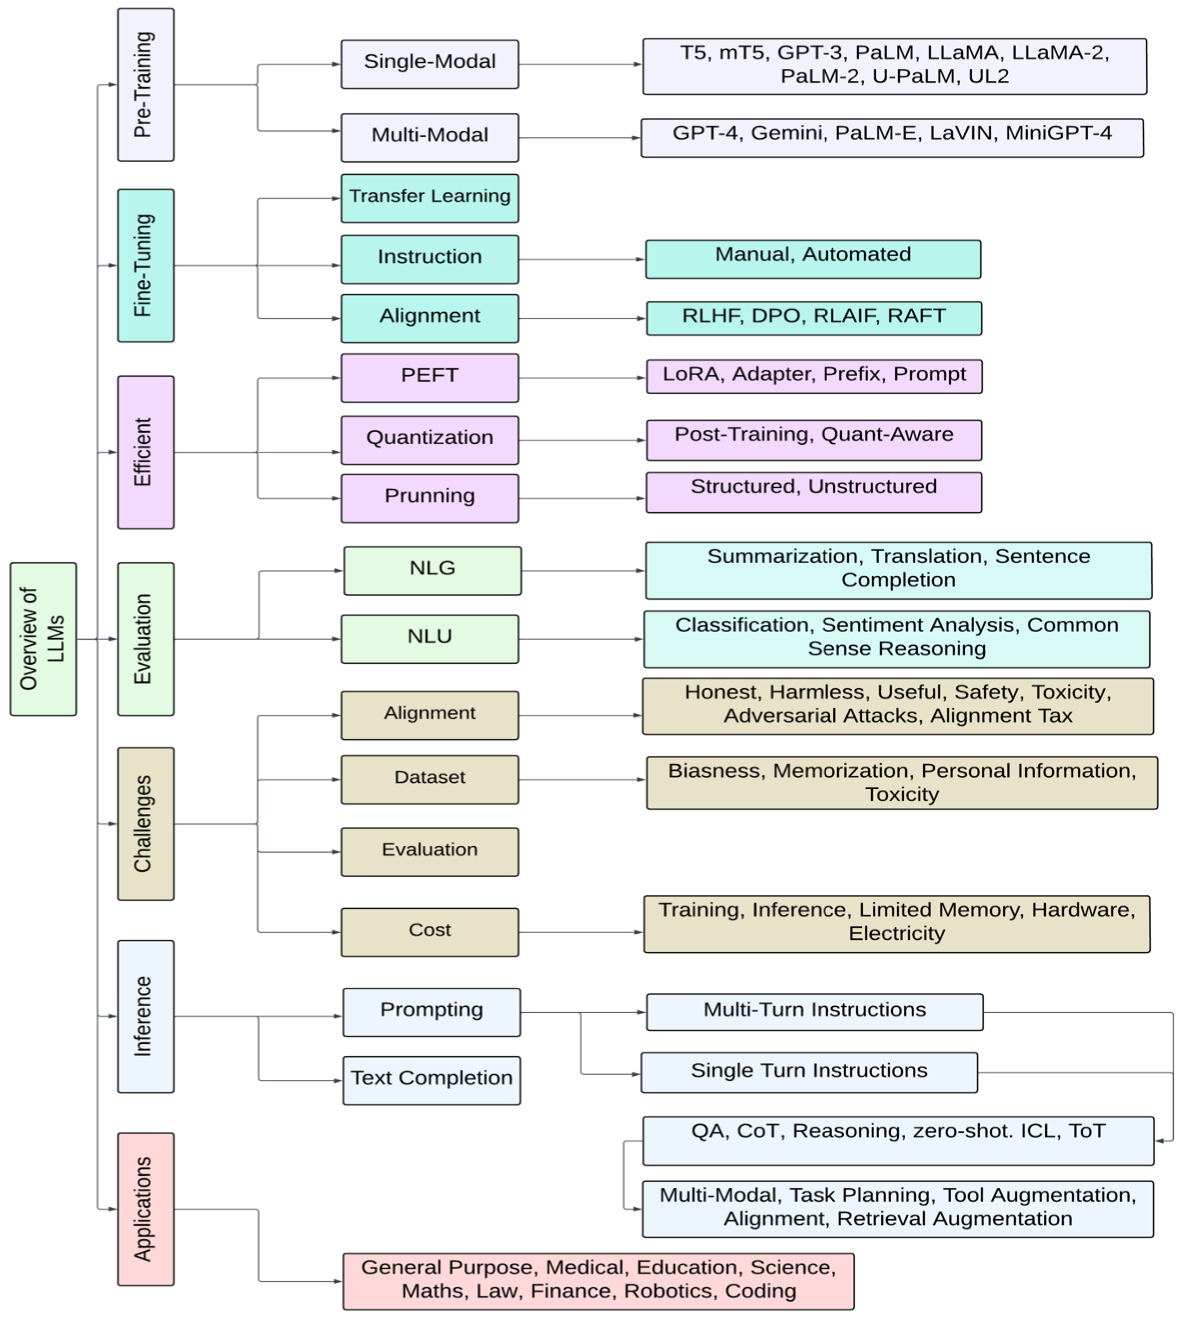
\includegraphics[width=0.8\textwidth]{03_Figures/literature-review/llms-overview.png}
     \rule{35em}{0.5pt}
    \caption{An overview of \glspl{llm} divided into seven branches: pre-training, fine-tuning, efficiency, evaluation, challenges, inference, and applications. (\cite{Naveed2023})}
 \label{fig:llms-overview}
\end{figure}

This adaptability has made \glspl{llm} suitable for tasks requiring contextual reasoning, dialogue systems, and even code generation, as seen in models like Codex (\cite{Chen2021EvaluatingLL}), which powers tools such as GitHub Copilot\footnote{\url{https://github.com/features/copilot}}.

The applications of \glspl{llm} span numerous domains, reflecting their versatility and broad impact.
In industry, \glspl{llm} power conversational agents, customer service bots, and content creation tools.
In research and education, they facilitate automated summarization of scientific literature, personalized tutoring, and question-answering systems to support knowledge discovery.
The integration of \glspl{llm} with domain-specific knowledge graphs and ontologies further enhances their reliability, particularly in specialized areas such as medicine, law, and scientific discovery (\cite{Yang2024}).

Despite their strengths, \glspl{llm} have some limitations.
One important problem is their dependence on vast computational resources for training, which has implications for environmental sustainability (\cite{Strubell2019EnergyAP}).
Furthermore, \glspl{llm} tend to propagate biases present in the training data, leading to inconsistencies when deployed in real-world applications (\cite{Naveed2023}).
They also suffer from factual inaccuracies and hallucinations, where the model generates plausible yet incorrect information (\cite{Chang2024}), which limits their applicability in high-stakes environments requiring factual precision.
Moreover, the lack of interpretability in \glspl{llm} remains a significant challenge, as their outputs are generated from complex internal representations that are not easily explainable, leading to questions about trust and accountability.

Nevertheless, the advantages of \glspl{llm} are substantial, as they offer unprecedented performance in language-related tasks, significant generalizability, and the ability to operate across diverse applications without extensive task-specific engineering.
In their study, \cite{Naveed2023} discuss that current research about \glspl{llm} efforts are focused on addressing their limitations, particularly improving energy efficiency, reducing bias, enhancing factual accuracy, and developing methods for better interpretability.
As \glspl{llm} continue to evolve, their integration with structured knowledge systems and advancements in alignment with human intent are likely to redefine their role in solving complex problems across industries.
%
\section{Recommender Systems}\label{sec:recommender-systems}
The task of recommender systems is to use users' data and their current and historical preferences with the goal of making predictions about users' possible future likes and interests \cite{Lu2012}.

In recommender systems, \gls{ml} models are used to predict the rating $r_{ui}$ of a user $u$ on an item $i$.
At inference time, the system recommends to each user $u$ the items $I$ having highest predicted rating $r_{ui}$.
It is therefore necessary to collect user feedback, so that we can have a ground truth for training and evaluating our models.
Explicit Feedback is a rating explicitly given by the user to express their satisfaction with an item.
Implicit Feedback assumes that user-item interactions are an indication of preferences.

The two main approaches in recommender systems are \gls{cbf} and \gls{cf}, often combined in hybrid methods \cite{Ko2022}.

\gls{cbf} is a method for recommending articles with attributes similar to those that users like and recommends them based on article information \cite{Vallet2006}.
According to \textcite{salter2006cinemascreen}, such filtering has a major drawback: it recommends only data on articles that are closely related to data on articles that a user has considered in the past. Because of this, the system struggles to recommend new articles. 

\gls{cf} relies on user-item interactions, such as ratings or clicks, to identify patterns and recommend items that were liked by similar users.
It is effective, but suffers from 3 problems such as: the sparsity problem, that occurs when there is not enough data available for recommendation \cite{Plexousakis2005}.
Another important problem is the cold start problem, which occurs when there is no evaluation data, that is, when a new user enters the system \cite{WEI201729}.
Finally, gray sheep is a problem in which there is only a small number of users with similar evaluation data to that of the individual user, and thus there are difficulties in providing recommendations \cite{Gras2016}.

Hybrid filtering systems integrate multiple recommendation techniques, such as \gls{cbf} and \gls{cf}, to address the shortcomings of each method and improve overall recommendation quality \cite{Ko2022}.
By combining these approaches, hybrid systems can utilize both item attributes and user behavior to create a more comprehensive understanding of preferences.
This combination enhances recommendation accuracy, increases diversity, and provides a more robust solution adaptable to various scenarios, making hybrid systems a superior choice for personalized recommendations.

\subsection*{Recommender Systems in Research Field}\label{sec:recommender-systems-in-research-field}
Most of the existing works of recommender systems in the literature regarding the field of research are based on suggesting research papers.
The following describes the work found during the literature review regarding these systems.

\textcite{refore} proposed the REFORE system, a hybrid recommender system specifically designed to assist researchers in managing information overload by providing high-quality and personalized recommendations of research papers.
The system integrates bibliometric measures, such as journal impact factors and author h-indexes, into its recommendation process, thereby emphasizing the quality of both the items (papers) and the users (researchers) involved.

REFORE employs a \gls{cbf} approach to match user preferences with paper content, using metadata such as keywords, abstracts, and citations.
It represents papers as vectors in a linguistic framework, assigning importance scores to keywords, which are then matched to user profiles.
The structure of the system is shown in Fig.~\ref{fig:refore}.
These profiles are built dynamically based on the researcher's past publications and manually input preferences.
Additionally, a collaborative filtering mechanism is implemented to leverage the feedback and preferences of similar users, identifying relevant items based on shared interests.

The system adopts a two-phase feedback process: users can evaluate recommendations as relevant or irrelevant and later provide qualitative assessments of the papers they read.
This feedback not only improves future recommendations but also helps refine the underlying quality measures for papers and authors.
A key innovation in REFORE is its re-ranking process, which combines \gls{cbf} and \gls{cf} outputs with quality scores derived from bibliometric data.
Papers are ranked not only by their relevance to the user but also by their scientific quality and novelty.

To handle the fuzziness inherent in user preferences and item quality, REFORE utilizes a fuzzy linguistic modeling approach, which ensures flexibility and granularity in assessing and aggregating preferences.
This linguistic framework allows for precise and interpretable measurements of similarities and quality across items and users.

\begin{figure}[htbp]
    \centering
 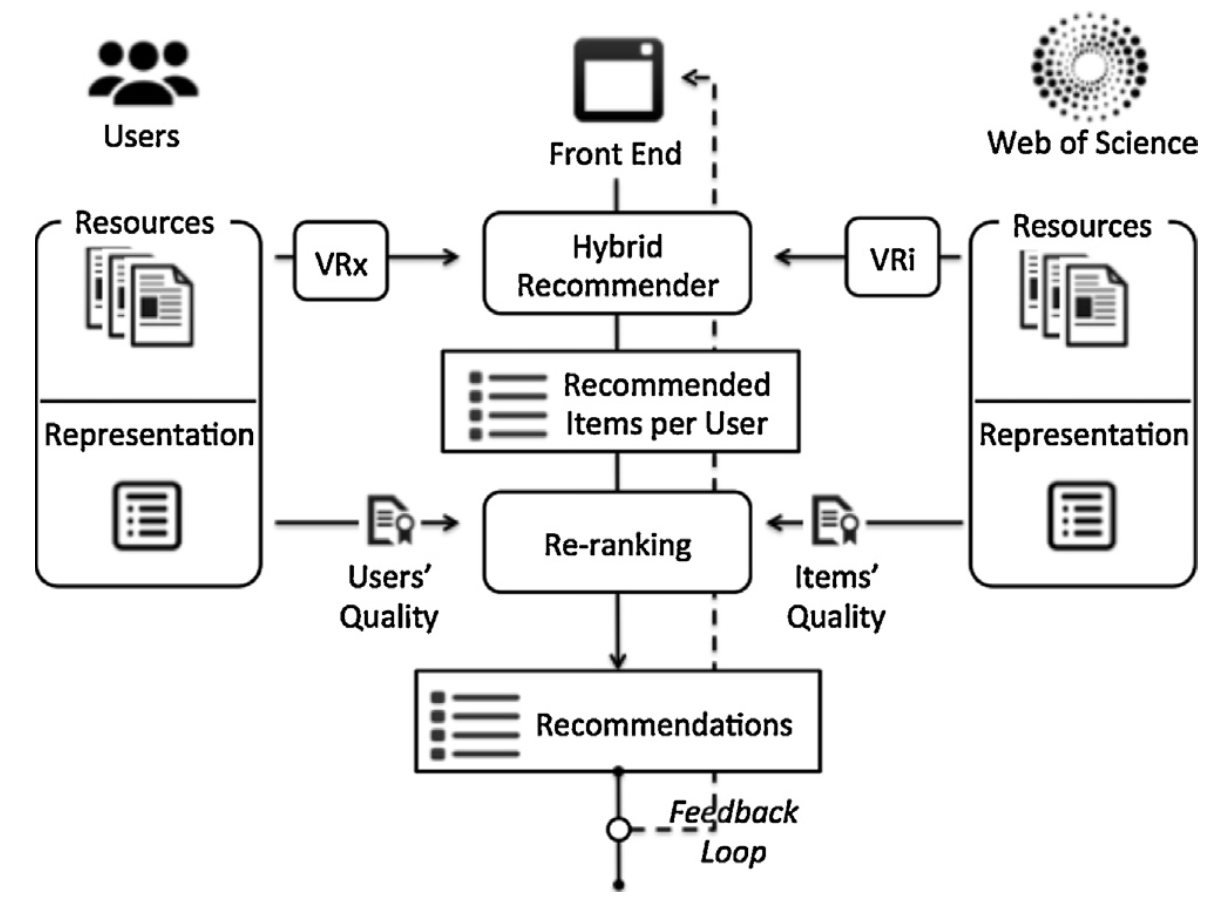
\includegraphics[width=0.8\textwidth]{03_Figures/literature-review/refore.png}
     \rule{35em}{0.5pt}
    \caption{Structure of REFORE system (\textcite{refore})}
 \label{fig:refore}
\end{figure}

In terms of evaluation, the system was tested with a group of researchers from multiple institutions over a year-long period.
Researchers received monthly recommendations based on newly published papers from the Web of Science database, and their feedback was collected to measure the system's effectiveness.
The experimental results demonstrated the system's ability to deliver high-quality and personalized recommendations, outperforming traditional methods by incorporating bibliometric quality measures and user feedback into the hybrid recommendation strategy.

\textcite{Kanwal2024} proposed a research paper recommendation system, integrating citation networks and collaboration networks to provide high-quality and relevant suggestions to researchers.
This approach, named \gls{rrmf}, addresses challenges such as the cold-start problem, data sparsity, and semantic ambiguity.

The proposed methodology involves generating a multi-level citation network, where the focal paper of interest (PI) serves as the central node.
Citation relationships are explored up to six levels, leveraging both forward (citing) and backward (cited by) links.
To evaluate the relevance of papers within the network, bibliographic coupling and co-citation strengths are computed, quantifying the similarity of papers based on shared citations or references.
A candidate score is derived for each paper, which is used to filter irrelevant documents and focus on those most closely related to the paper of interest.

Additionally, centrality measures (such as betweenness, degree, closeness, and eigenvector centrality) are applied to rank papers based on their structural significance within the network.
Papers with high centrality scores are selected for further analysis.

The system extends beyond citation networks by incorporating collaboration networks of authors.
Authors are extracted from top-ranked papers, and their collaboration networks are analyzed using centrality and social measures to identify influential researchers.
These author-based insights contribute to refining paper recommendations, ensuring that suggested papers come from prominent authors within the field.

To evaluate the system, the AMiner dataset, comprising nearly 4.8 million papers and over 45 million citation relationships, was used.
The system's performance was benchmarked using metrics such as \gls{map}, \gls{mrr}, and \gls{ndcg}.
Experimental results demonstrated that the \gls{rrmf} outperformed traditional systems, such as Google Scholar and previous citation-based methods, by achieving higher precision and recall.
The incorporation of multi-level citation analysis and author collaboration measures significantly improved the quality and relevance of recommendations.

\textcite{Murali2019} proposed a research paper recommender system using a user-based collaborative filtering approach.
The goal of the system is to recommend research papers tailored to a user's interests by analyzing their preferences and similarities with other users.
The authors addressed the challenge of information overload faced by researchers due to the rapid growth in the number of research publications.

The system operates by collecting a dataset of user-paper interactions, which includes attributes such as user IDs, paper IDs, and ratings assigned by users to the papers. Based on this data, the system calculates the similarity between users using the cosine similarity measure. This approach evaluates the resemblance between user profiles by treating their preferences as vectors and computing the cosine of the angle between them.
Users with similar interests are identified, and recommendations are generated by predicting ratings for papers based on the ratings given by these similar users.
The block diagram of the system architecture is shown in Fig.~\ref{fig:murali}.

To improve the quality of recommendations, the system utilizes a prediction rating mechanism, which assigns a predicted score to papers based on the collaborative filtering model.
Papers with higher predicted ratings are recommended to the user, ensuring that suggestions align with their preferences.
The authors also implemented a ``user-link formation'' step to construct the collaborative filtering model, leveraging the collective behavior of similar users to refine recommendations further.

\begin{figure}[htbp]
    \centering
 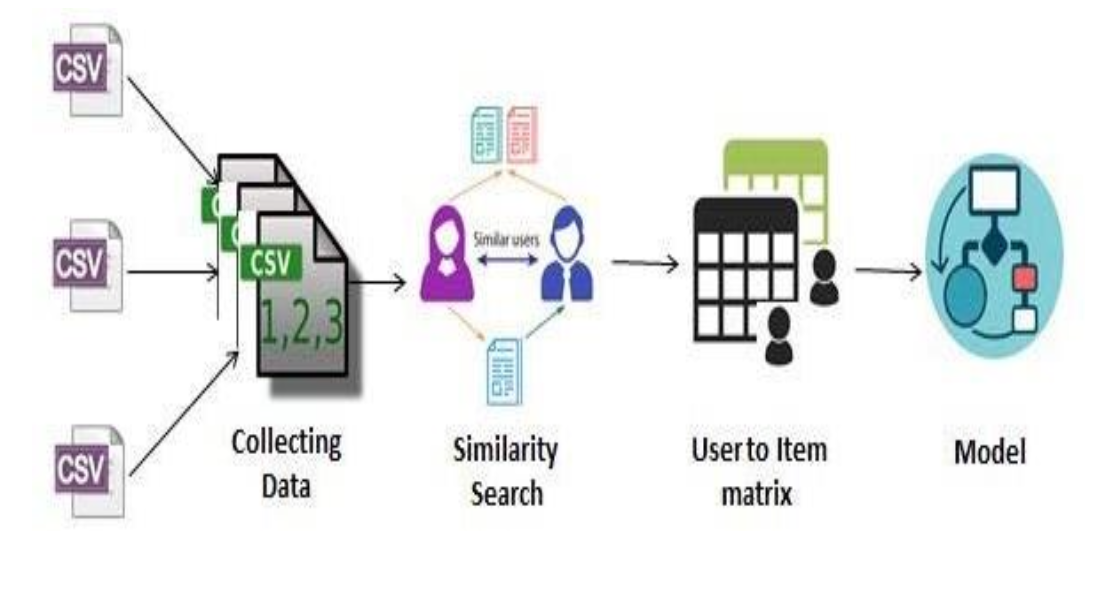
\includegraphics[width=0.8\textwidth]{03_Figures/literature-review/murali.png}
     \rule{35em}{0.5pt}
    \caption{Block diagram of the system architecture (\textcite{Murali2019})}
 \label{fig:murali}
\end{figure}

For evaluation, the system was tested on a dataset comprising 135 users and their interactions with research papers.
Performance was measured using metrics like \gls{mae} and \gls{rmse} to assess the accuracy of predicted ratings against actual ratings.
The results showed that the user-based collaborative filtering model performed well, producing high-quality recommendations with minimal deviation in predicted ratings.
The authors acknowledge limitations in their work, such as the reliance on a synthetic dataset for testing due to the unavailability of real-world datasets with pre-existing paper ratings.
They suggest that the system's effectiveness could be further enhanced if real datasets from platforms like research paper repositories were used.

In their work, \textcite{Sharma2023} present a detailed exploration of research paper recommender systems, addressing their evolution, methodologies, and associated challenges.
It categorizes existing approaches into key methodologies, including \gls{cbf}, \gls{cf}, link-based algorithms, co-occurrence techniques, and hybrid approaches.
Each method is analyzed based on its underlying knowledge sources, such as textual attributes of research papers, author profiles, citation patterns, and user-generated tags, which are leveraged to model user preferences and generate personalized recommendations.
Based on their studies, the authors divide recommender systems into three essential components: the first requirement for performing any task is domain-specific knowledge and its application to the task at hand.
This is called principle or basic knowledge and operational theory.
Principle knowledge includes all available information about an item that is used to perform the recommendation task and serves as key attributes of the system to generate recommendations.
Operational theory, on the other hand, is concerned with the ``how'' aspect, i.e., how the information provided is applied to achieve the intended goals.
The second component is the recommendation approach, which outlines a step-by-step methodology for solving the problem, detailing implementation techniques and their practical implementation.
Finally, the third component, probably the most critical, is user modeling.
The general architecture of a research paper recommendation system is shown in Fig.~\ref{fig:general-architecture-rprs}.

\begin{figure}[htbp]
    \centering
 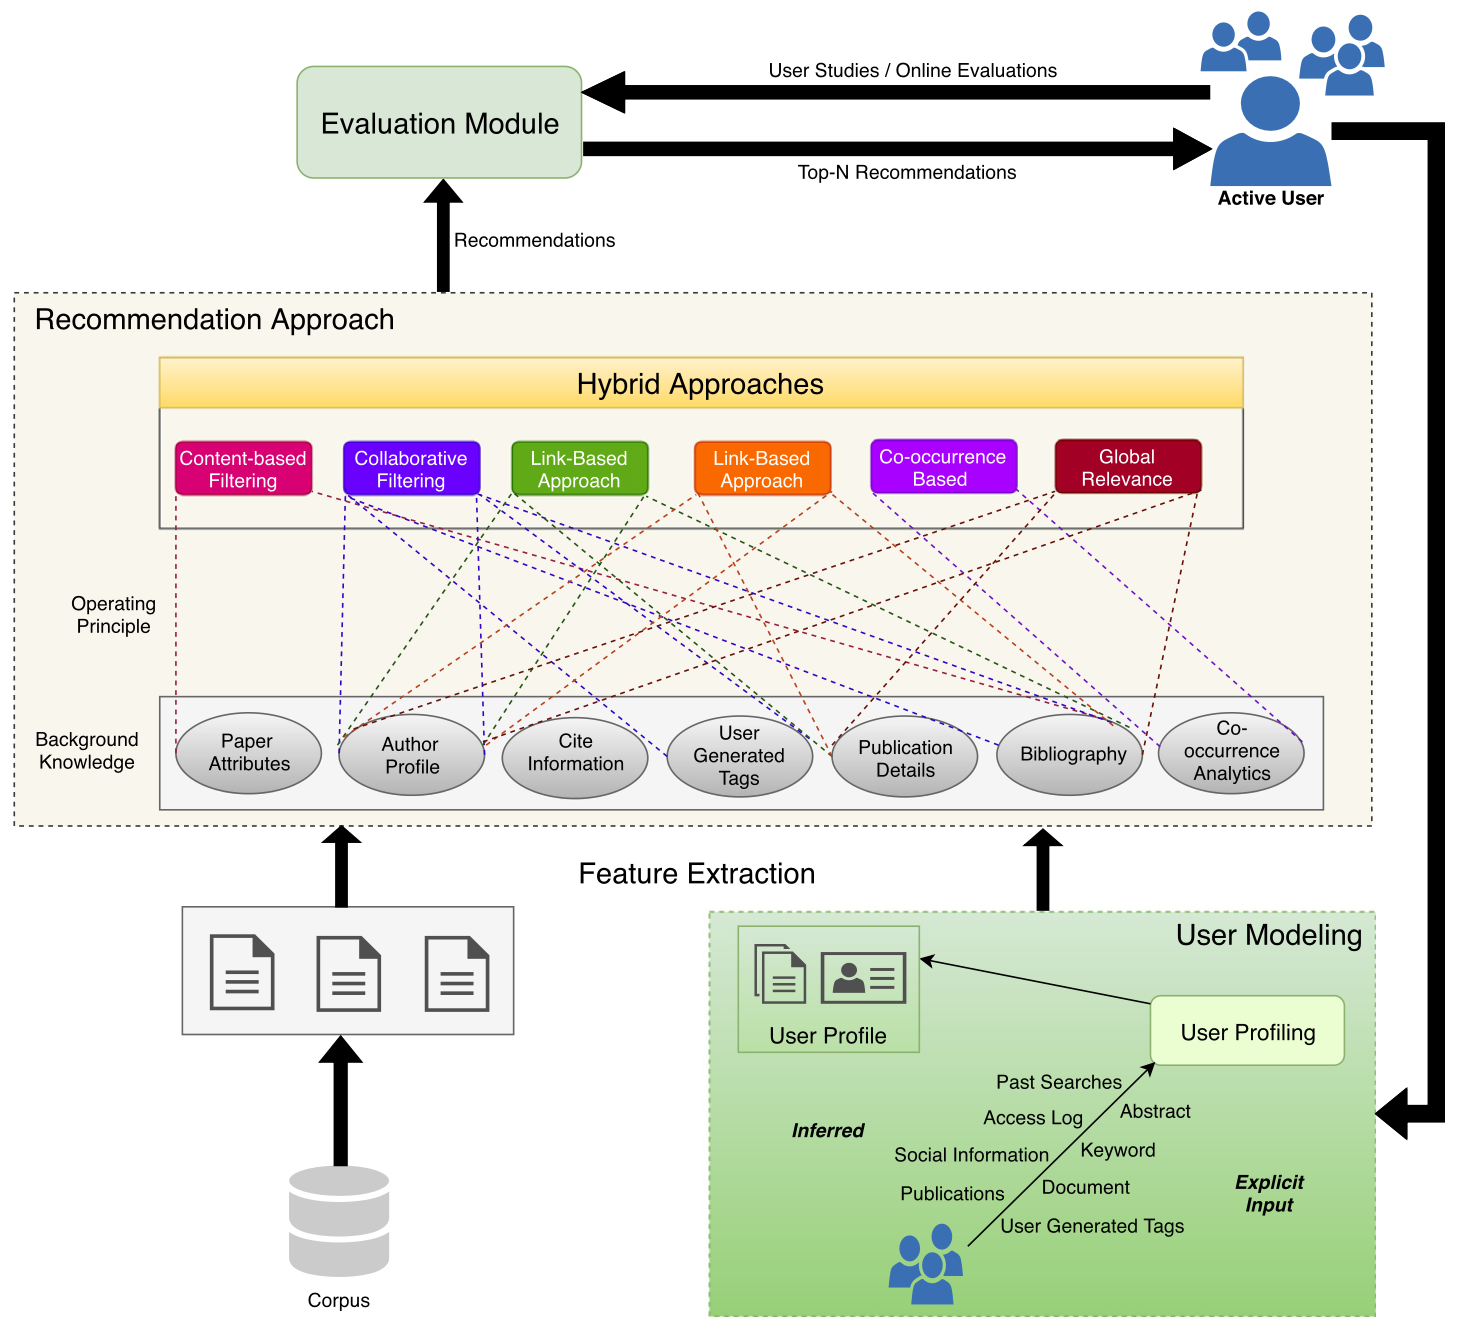
\includegraphics[width=0.8\textwidth]{03_Figures/literature-review/general-architecture-rprs.png}
     \rule{35em}{0.5pt}
    \caption{General architecture of Research Paper Recommendation System (\textcite{Sharma2023})}
 \label{fig:general-architecture-rprs}
\end{figure}

The authors highlight the dominance of \gls{cbf} techniques, which rely on textual similarity between papers and user profiles, and discuss how \gls{cf} leverages peer preferences to improve recommendations.
Hybrid methods, which integrate multiple approaches, are presented as a solution to address the limitations of individual techniques, such as over-specialization in \gls{cbf} and data sparsity in \gls{cf}.
The study also identifies critical challenges, including the lack of standard datasets for benchmarking, insufficient evaluation metrics for dimensions like novelty and serendipity, and the difficulty of scaling algorithms to handle real-world, large-scale datasets.
Furthermore, the paper underscores the need for more sophisticated evaluation frameworks and advanced computational models, such as \gls{dl}, to improve the efficacy and scalability of research paper recommender systems.

\textcite{Jagadishwari2023} proposed a methodology for recommending academic collaborators using a combination of citation analysis and academic influence metrics.
Their work highlights the importance of identifying suitable collaborators to enhance research productivity and addresses the challenges posed by the vast volume of academic data.
The system utilizes the DBLP dataset \cite{Ley2002}, focusing on core computer science publications from 2017 to 2019, and incorporates citation count and influential citation metrics to assess academic influence.

The methodology involves preprocessing the dataset to eliminate irrelevant data, computing an Academic Level Index (ALI) using three different formulae, and then calculating a Research Score (R score) based on ALI and domain-specific publication metrics.
The R score serves as the basis for ranking scholars and identifying potential collaborators.
Three variations of the R score computation are tested, and the study concludes that the third formula (R3 Score) yields the most compatible recommendations by minimizing differences between the scores of the target scholar and recommended collaborators.
The system's results are visualized using graphs and compared across the three scoring methods, demonstrating that R3 Score provides the most precise matches.
The authors suggest future research could include additional factors like geographic location and funding status, as well as expanding the dataset to other academic disciplines.

\textcite{Zhang2023} provide a comprehensive review of scholarly recommendation systems, highlighting their evolution, methodologies, applications, and challenges.
These systems play a crucial role in academia, assisting researchers in identifying relevant literature, potential collaborators, conferences, journals, datasets, and grant opportunities.
The study identifies \gls{cbf} as the most widely used technique, particularly for literature recommendations, whereas \gls{cf} is more prevalent in conference and collaborator recommenders.
Hybrid approaches, which combine \gls{cbf} and \gls{cf}, are also discussed as a promising direction for improving recommendation accuracy and diversity.

The paper evaluates 225 publications across various SRS domains, showing that literature and collaborator recommendation systems dominate the field, while systems for datasets and grants are underexplored.
It notes the limited adoption of deep learning methods in scholarly recommendation systems and emphasizes the need for better integration of user feedback mechanisms to enhance system personalization and effectiveness.
Furthermore, the study highlights the challenges of scalability, data sparsity, and the cold start problem in existing systems.
Evaluation methods, including online and offline metrics, are examined, with offline evaluations being the most common.
In its conclusion, the paper stresses the importance of developing unified frameworks that integrate diverse methodologies and leverage advances in \gls{ai} to address current limitations.
It also calls for more research into underrepresented areas like dataset and grant recommendation systems, advocating for user-centric designs that prioritize usability and practical application.

\textcite{Du2022} proposed a novel model called ACR-ANE to enhance the recommendation of academic collaborators by integrating network topology and multi-type scholar attributes.
The study addresses the limitations of existing approaches, which often consider only local network structures or singular attribute types, and introduces non-local neighbors to capture stronger academic relationships.
Non-local neighbors are determined through biased random walks and frequency filtering, allowing the model to identify significant connections beyond immediate collaborators.

The methodology incorporates six scholarly attributes-academic age, research interests, publication count, average citations, number of collaborators, and H-index—into a scholar attribute matrix.
These attributes, combined with network structure, are encoded using a deep auto-encoder to generate low-dimensional embeddings that preserve both local and global academic network characteristics.
The model establishes a new multi-type relational network by integrating non-local neighbors and attribute-based proximity, which enriches the representation of academic relationships.
The framework of ACR-ANE is shown in Fig.~\ref{fig:acr-ane}.

\begin{figure}[htbp]
    \centering
 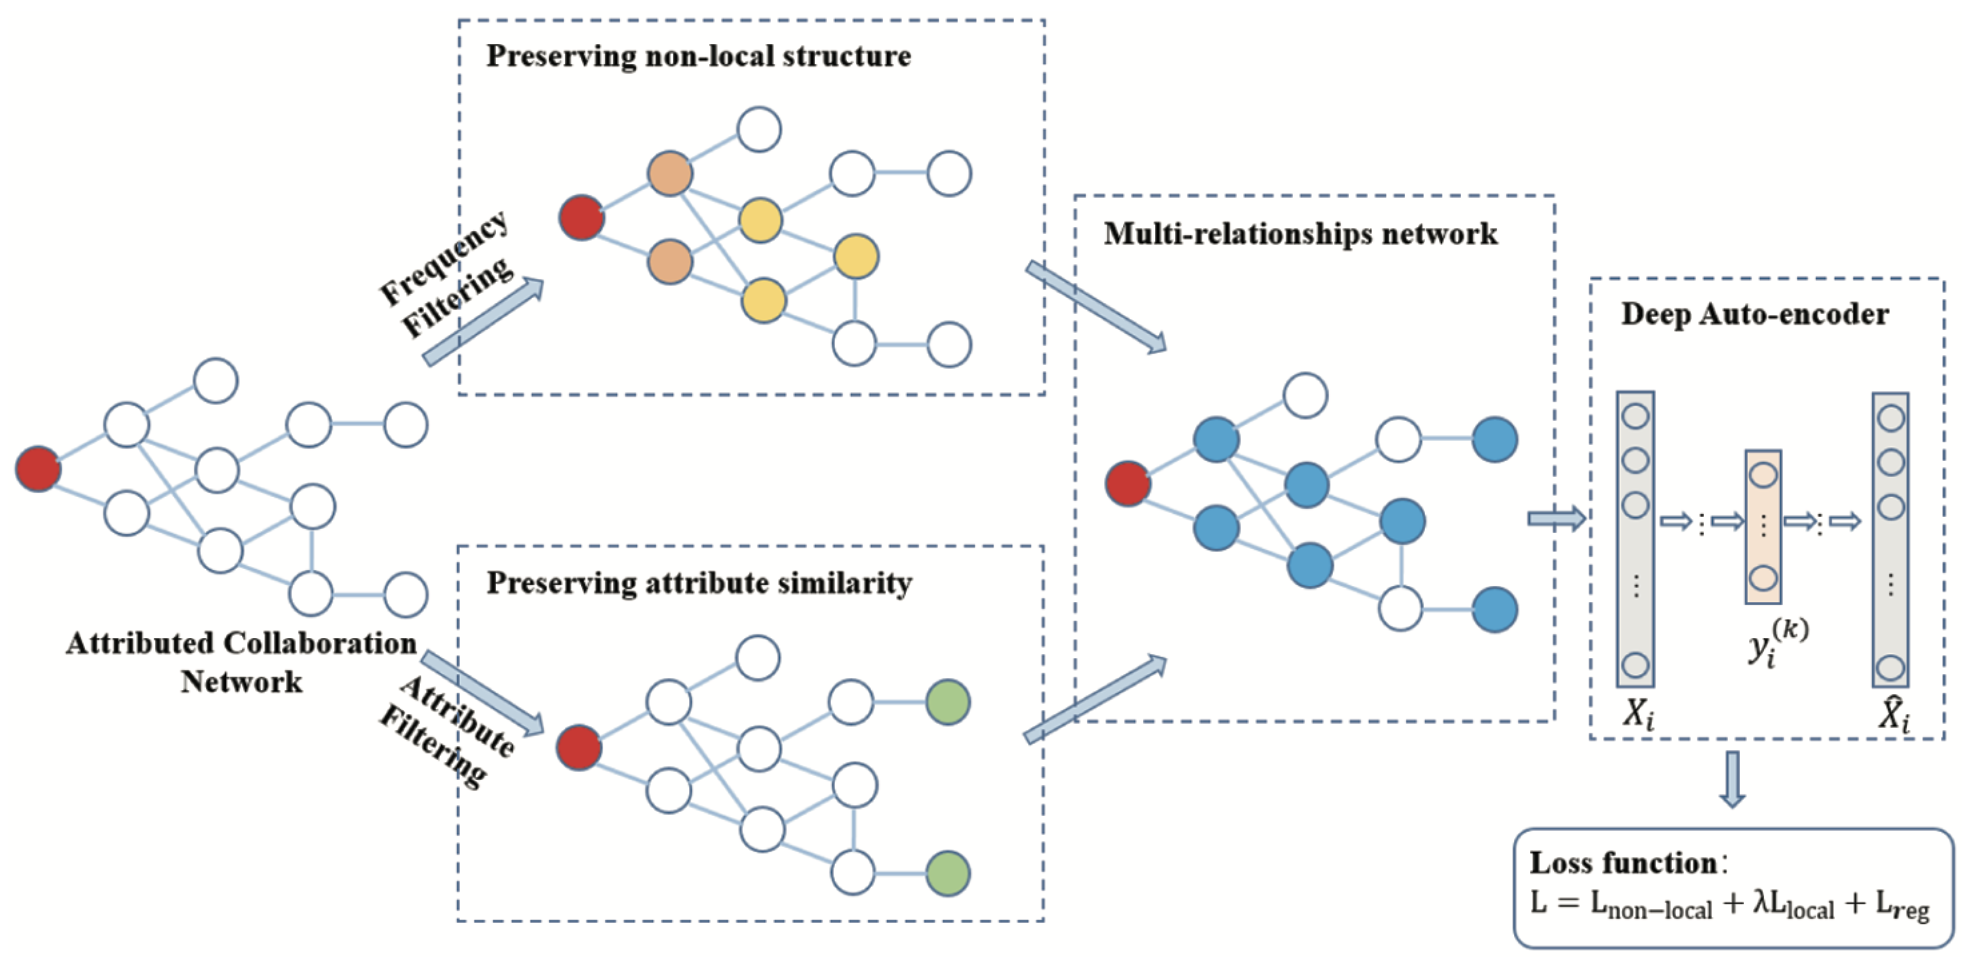
\includegraphics[width=0.8\textwidth]{03_Figures/literature-review/academic-collaborator-recommendation-framework.png}
     \rule{35em}{0.5pt}
    \caption{The framework of ACR-ANE model. (\textcite{Du2022})}
 \label{fig:acr-ane}
\end{figure}

Extensive experiments conducted on two real-world datasets, Aminer and APS, demonstrate the superior performance of ACR-ANE in comparison to baseline models such as DeepWalk, TADW, SDNE, and ACNE.
The results highlight the effectiveness of combining network structure and scholar attributes for collaborator recommendation.
However, the study acknowledges its limitation in handling dynamic networks and suggests future work on incorporating temporal factors to reflect evolving academic collaborations.


\textcite{Zhu2022} explored the application of \glspl{gnn} to recommend research collaborators in the academic domain.
The study focuses on leveraging dynamic and temporal aspects of research networks, addressing the challenge of identifying suitable collaborators in a rapidly evolving academic landscape.
The authors utilize data from the MEDLINE database and implement two \gls{gnn}-based models, GraphSAGE and \gls{tgn}, to capture both static and temporal dependencies among researchers.

GraphSAGE employs an inductive approach that generates embeddings for unseen nodes by aggregating neighbor features, making it suitable for large and dynamic graphs.
\gls{tgn} extends this by incorporating temporal elements, using a message-passing mechanism to update node embeddings based on time-stamped interactions.
These models are compared against baseline methods, including the transductive LightGCN and a \gls{gbc}.

The study is divided into two experimental scenarios: automatic evaluations using \gls{auc} and average precision metrics, and external evaluations based on user ratings collected via a web-based application.
Results indicate that TGN outperforms other methods in handling temporal dynamics and inductive tasks, particularly when using publication titles as node features. While GraphSAGE exhibits strong performance for static embeddings, TGN demonstrates superior capability in predicting future collaborations by integrating time-sensitive relationships.

The authors acknowledge limitations such as the small sample size in external evaluations and the reliance on static node features for some tests.
They propose future enhancements, including the integration of distribution-based representations for nodes to better manage uncertainty and improve predictive modeling.

\subsection*{Retrieval-Augmented Recommender Systems}\label{sec:retrieval-augmented-recommender-systems-in-research-field}

According to \textcite{Deldjoo2024}, \gls{rag} leverages the integration of retrieval systems and generative models to produce highly relevant and context-aware recommendations.
This approach stores knowledge externally, allowing dynamic updates and reducing the risk of hallucinations by grounding outputs in retrieved data.
By minimizing the need for extensive model parameters, \gls{rag} improves efficiency and makes complex tasks, such as generating personalized explanations, more feasible.
However, its effectiveness is strictly linked to the quality and relevance of the retrieved information, making it reliant on robust retrieval systems and well-curated external knowledge bases.
Additionally, the integration of retrieval and generation components introduces complexity and potential computational overhead, especially in real-time applications.
Despite these challenges, \gls{rag} offers a powerful framework for enhancing the accuracy and adaptability of modern recommender systems.

For example, \textcite{Banerjee2024} propose an approach to improving tourism recommender systems by integrating sustainability considerations into the recommendation process.
The authors leverage \gls{rag} to enhance \glspl{llm} for generating recommendations, focusing on sustainable city trips in Europe.
Their main innovation is the incorporation of a sustainability metric during the \gls{rag} pipeline's prompt augmentation phase, called Sustainability Augmented Reranking (SAR).

Fig.~\ref{fig:sar-enhanced-recommendation} illustrates the SAR-enhanced recommendation process, which adjusts the traditional \gls{rag} pipeline by including a sustainability metric based on city popularity and seasonal demand.

\begin{figure}[htbp]
    \centering
    \rule{35em}{0.5pt}
    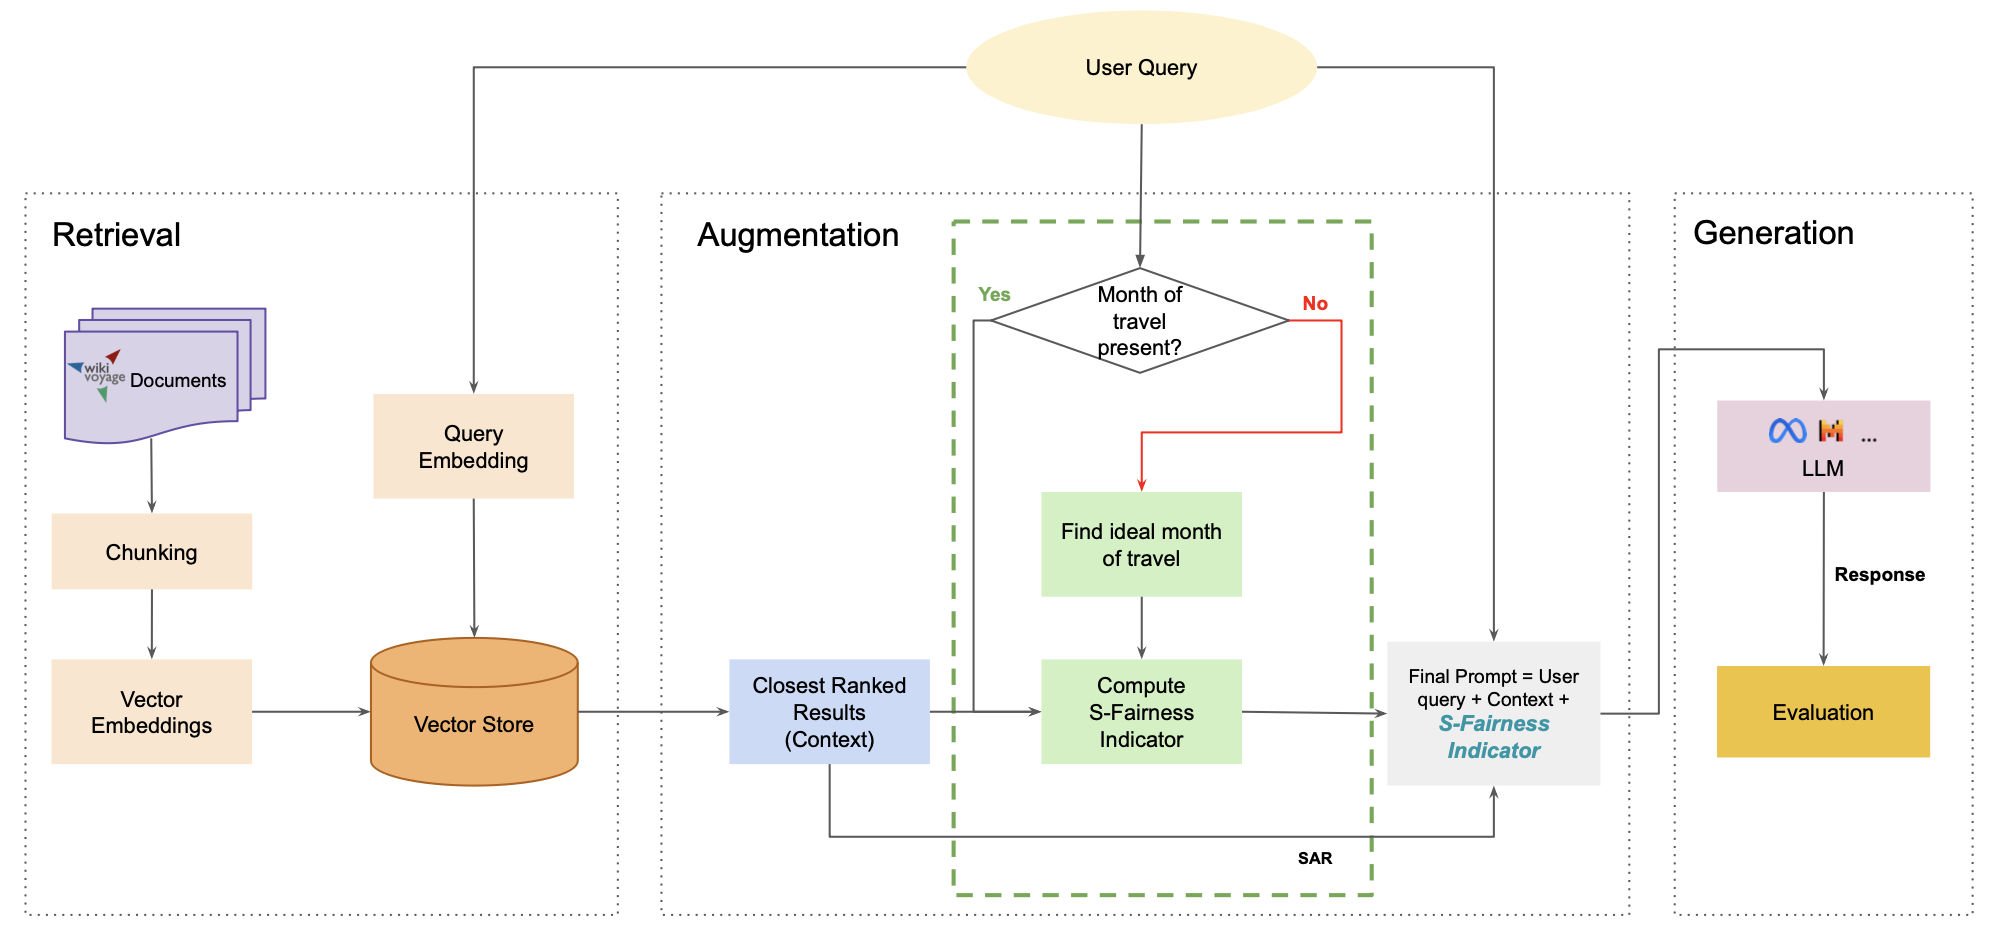
\includegraphics[width=0.8\textwidth]{03_Figures/literature-review/rag-tourism.png}
    \caption{SAR-enhanced recommendation process (\textcite{Banerjee2024})}
 \label{fig:sar-enhanced-recommendation}
\end{figure}

The SAR enhancement adjusts the traditional \gls{rag} process by including a sustainability metric based on city popularity and seasonal demand.
This metric helps the system prioritize recommendations that align with sustainability principles, such as promoting destinations with lower tourism pressure during certain months.
By leveraging data from sources like Wikivoyage\footnote{\url{https://www.wikivoyage.org}} and Tripadvisor\footnote{\url{https://www.tripadvisor.com}}, the system calculates popularity and seasonality indices to inform the SAR metric, ensuring that recommendations balance user preferences with environmental and societal considerations.

Using open-source \glspl{llm}, such as Llama-3.1-Instruct-8B and Mistral-Instruct-7B, the study demonstrates that SAR-enhanced recommendations perform equal to or better than baseline models (without SAR) in terms of quality and sustainability.
The approach reduces common issues in \gls{llm}-based TRS, like hallucinations, and supports a multi-stakeholder perspective by addressing the needs of users, local communities, and environmental sustainability.

Another example is \gls{ramo}, a system designed to enhance Massive Open Online Courses (MOOCs) recommendations by addressing the ``cold start'' problem common in recommender systems \cite{Rao2024}.
Traditional course recommendation systems often struggle with new users due to the absence of historical data.
\gls{ramo} tackles this limitation by leveraging a \gls{rag} pipeline integrated with \gls{llm}.

In \gls{ramo}, the \gls{rag} framework combines two key components: a retriever and a generator.
The retriever accesses a pre-built knowledge base of course data, such as Coursera's publicly available dataset, and retrieves relevant information based on user queries.
The retrieved content is used to augment the prompts provided to the generator, ensuring responses are contextually relevant and precise.
This setup enables \gls{ramo} to generate personalized course recommendations even when little or no user-specific information is available, thereby overcoming the cold start issue.

The \gls{ramo} system workflow is shown in Fig.~\ref{fig:ramo-system-workflow}.

\begin{figure}[htbp]
    \centering
    \rule{35em}{0.5pt}
    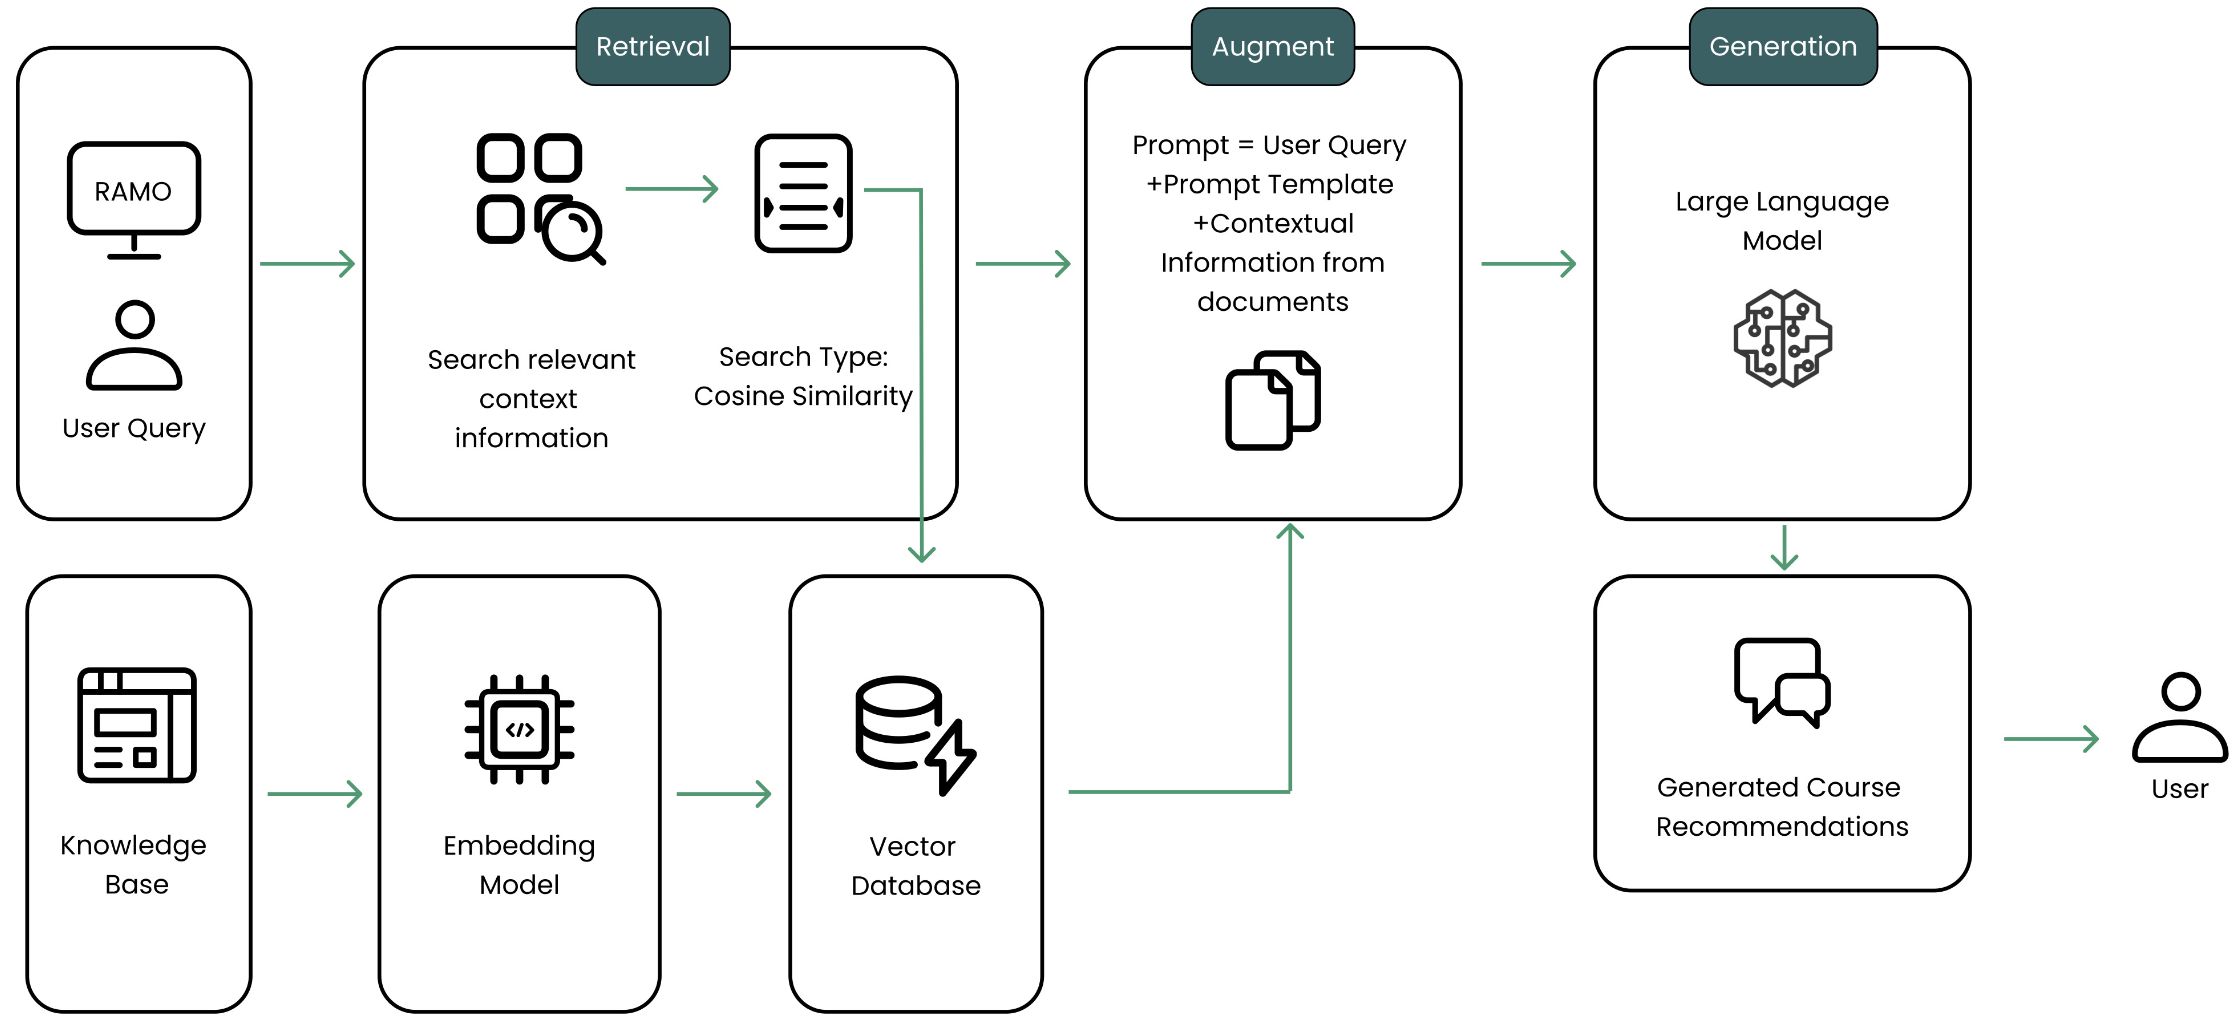
\includegraphics[width=0.8\textwidth]{03_Figures/literature-review/ramo.png}
    \caption{The \gls{ramo} System workflow (\textcite{Rao2024})}
 \label{fig:ramo-system-workflow}
\end{figure}

The system utilizes advanced text embedding techniques to store and retrieve course data efficiently, employing models like OpenAI's text-embedding-ada-002 for embedding generation.
The final recommendations are produced by GPT-3.5 Turbo, selected for its cost-efficiency and performance, allowing dynamic, conversational interaction with users.

The paper evaluates \gls{ramo} by comparing its performance to traditional systems and standard \gls{llm}-based recommenders without \gls{rag}.
Results show that the \gls{rag}-enhanced system delivers more personalized and flexible recommendations, particularly in scenarios requiring personalized suggestions or dealing with general queries from new users.
The integration of \gls{rag} also ensures that the recommendations align closely with user needs by dynamically retrieving and incorporating domain-specific knowledge.
%\fillingPage{}
%\chapter{Research Design}\label{chap:research-method}

\section{Research Philosophy}\label{sec:research-philosophy}
%
\section{Research Approach}\label{sec:research-approach}
%
\section{Methodology}\label{sec:methodology}
%
\section{Research Strategy}\label{sec:research-strategy}
%
\section{Data Collection}\label{sec:data-collection}
%
\section{Data Analysis}\label{sec:data-analysis}
\fillingPage{} 
\chapter{Conclusion}\label{chap:conclusion}

%----------------------------------------------------------------------------------------
%	BIBLIOGRAPHY
%----------------------------------------------------------------------------------------

\fillingPage{}
\nocite{*}
\listOfBibliography

%----------------------------------------------------------------------------------------
%	GLOSSARY (if appropriate)
%----------------------------------------------------------------------------------------

% \fillingPage{}
% \listOfGlossary

%----------------------------------------------------------------------------------------
%	ABBREVIATIONS (if appropriate)
%----------------------------------------------------------------------------------------
\fillingPage{}
\listOfAbbreviation

%%----------------------------------------------------------------------------------------
%%	LIST OF FIGURES (optional)
%%----------------------------------------------------------------------------------------

\fillingPage{} 
\listOfFigures

%%----------------------------------------------------------------------------------------
%%	LIST OF TABLES (optional)
%%----------------------------------------------------------------------------------------

\fillingPage{} 
\listOfTables

%----------------------------------------------------------------------------------------
%	THESIS CONTENT - APPENDICES (if appropriate)
%----------------------------------------------------------------------------------------

\appendix % Cue to tell LaTeX that the following 'chapters' are Appendices

% Include the appendices of the thesis as separate files from the Appendices folder
% Uncomment the lines as you write the Appendices

% \fillingPage{} 
% % Appendix A

\chapter{Appendix Title Here} % Main appendix title

\label{AppendixA} % For referencing this appendix elsewhere, use \ref{AppendixA}

\addtocontents{toc}{\vspace{1em}} % Add a gap in the Contents, for aesthetics

Write your Appendix content here.

% \fillingPage{} 
% % Appendix A

\chapter{Appendix Title Here} % Main appendix title

\label{AppendixB} % For referencing this appendix elsewhere, use \ref{AppendixA}

\addtocontents{toc}{\vspace{1em}} % Add a gap in the Contents, for aesthetics

Write your Appendix content here.

%\fillingPage{} 
%\input{02_Appendices/AppendixC}

%----------------------------------------------------------------------------------------
%	FOREWORD / ACKNOWLEDGEMENTS (optional)
%----------------------------------------------------------------------------------------

\ackPage{
    The acknowledgements and the people to thank go here, don't forget to include your project advisor\ldots
}

\clearpage % Start a new page

\backmatter

\end{document}  